% 1) pdflatex main
% 2) makeindex main.idx -s StyleInd.ist
% 3) biber main
% 4) pdflatex main x 2

\documentclass[11pt,fleqn]{book} % Default font size and left-justified equations
\usepackage[top=3cm,bottom=3cm,left=3.2cm,right=3.2cm,headsep=10pt,a4paper]{geometry} % Page margins
\usepackage{xcolor} % Required for specifying colors by name
%\definecolor{ocre}{RGB}{0.16,0.32,0.75}
\definecolor{ocre}{RGB}{243,102,25} % Define the orange color used for highlighting throughout the book
% Font Settings
\usepackage{avant} % Use the Avantgarde font for headings
%\usepackage{times} % Use the Times font for headings
\usepackage{mathptmx} % Use the Adobe Times Roman as the default text font together with math symbols from the Sym­bol, Chancery and Com­puter Modern fonts
\usepackage{microtype} % Slightly tweak font spacing for aesthetics
\usepackage[utf8]{inputenc} % Required for including letters with accents
\usepackage[T1]{fontenc} % Use 8-bit encoding that has 256 glyphs
\usepackage{amsmath,amssymb,amsfonts,latexsym}
\usepackage{latexsym}
\usepackage{amsmath}
\usepackage{amsfonts}
\usepackage[spanish]{babel}
\usepackage{mathrsfs}
\usepackage{psfrag}
\usepackage{graphicx}
\usepackage{amssymb}
\usepackage{multirow}
\usepackage{rotating}
\usepackage{enumerate}

\usepackage{cancel}

\usepackage{subfig}%PARA LAS FIGURAS MULTIPLES
\usepackage{multicol}


%\usepackage{enumitem}
%\usepackage[version=3]{mhchem}


\usepackage[spanish]{babel}

\spanishdecimal{.} %PARA EL PUNTO DECIMAL


% Index
\usepackage{calc} % For simpler calculation - used for spacing the index letter headings correctly
\usepackage{makeidx} % Required to make an index
\makeindex % Tells LaTeX to create the files required for indexing
%----------------------------------------------------------------------------------------

%----------------------------------------------------------------------------------------
%	VARIOUS REQUIRED PACKAGES
%----------------------------------------------------------------------------------------

\usepackage{titlesec} % Allows customization of titles

\usepackage{graphicx} % Required for including pictures
\graphicspath{{Pictures/}} % Specifies the directory where pictures are stored

\usepackage{lipsum} % Inserts dummy text

\usepackage{tikz} % Required for drawing custom shapes

\usepackage[spanish]{babel} % english language/hyphenation

\usepackage{enumitem} % Customize lists
\setlist{nolistsep} % Reduce spacing between bullet points and numbered lists

\usepackage{booktabs} % Required for nicer horizontal rules in tables

\usepackage{eso-pic} % Required for specifying an image background in the title page

%----------------------------------------------------------------------------------------
%	MAIN TABLE OF CONTENTS
%----------------------------------------------------------------------------------------

\usepackage{titletoc} % Required for manipulating the table of contents

\contentsmargin{0cm} % Removes the default margin
% Chapter text styling
\titlecontents{chapter}[1.25cm] % Indentation
{\addvspace{15pt}\large\sffamily\bfseries} % Spacing and font options for chapters
{\color{ocre!60}\contentslabel[\Large\thecontentslabel]{1.25cm}\color{ocre}} % Chapter number
{}
{\color{ocre!90}\normalsize\sffamily\bfseries\;\titlerule*[.5pc]{.}\;\thecontentspage} % Page number
% Section text styling
\titlecontents{section}[1.25cm] % Indentation
{\addvspace{5pt}\sffamily\bfseries} % Spacing and font options for sections
{\contentslabel[\thecontentslabel]{1.25cm}} % Section number
{}
{\sffamily\hfill\color{black}\thecontentspage} % Page number
[]
% Subsection text styling
\titlecontents{subsection}[1.25cm] % Indentation
{\addvspace{1pt}\sffamily\small} % Spacing and font options for subsections
{\contentslabel[\thecontentslabel]{1.25cm}} % Subsection number
{}
{\sffamily\;\titlerule*[.5pc]{.}\;\thecontentspage} % Page number
[]

%----------------------------------------------------------------------------------------
%	MINI TABLE OF CONTENTS IN CHAPTER HEADS
%----------------------------------------------------------------------------------------

% Section text styling
\titlecontents{lsection}[0em] % Indendating
{\footnotesize\sffamily} % Font settings
{}
{}
{}

% Subsection text styling
\titlecontents{lsubsection}[.5em] % Indentation
{\normalfont\footnotesize\sffamily} % Font settings
{}
{}
{}

%----------------------------------------------------------------------------------------
%	PAGE HEADERS
%----------------------------------------------------------------------------------------

\usepackage{fancyhdr} % Required for header and footer configuration

\pagestyle{fancy}
\renewcommand{\chaptermark}[1]{\markboth{\sffamily\normalsize\bfseries #1}{}} % Chapter text font settings
\renewcommand{\sectionmark}[1]{\markright{\sffamily\normalsize\thesection\hspace{5pt}#1}{}} % Section text font settings
\fancyhf{} \fancyhead[LE,RO]{\sffamily\normalsize\thepage} % Font setting for the page number in the header
\fancyhead[LO]{\rightmark} % Print the nearest section name on the left side of odd pages
\fancyhead[RE]{\leftmark} % Print the current chapter name on the right side of even pages
\renewcommand{\headrulewidth}{0.5pt} % Width of the rule under the header
\addtolength{\headheight}{2.5pt} % Increase the spacing around the header slightly
\renewcommand{\footrulewidth}{0pt} % Removes the rule in the footer
\fancypagestyle{plain}{\fancyhead{}\renewcommand{\headrulewidth}{0pt}} % Style for when a plain pagestyle is specified

% Removes the header from odd empty pages at the end of chapters
\makeatletter
\renewcommand{\cleardoublepage}{
\clearpage\ifodd\c@page\else
\hbox{}
\vspace*{\fill}
\thispagestyle{empty}
\newpage
\fi}

%----------------------------------------------------------------------------------------
%	THEOREM STYLES
%----------------------------------------------------------------------------------------

\usepackage{amsmath,amsfonts,amssymb,amsthm} % For including math equations, theorems, symbols, etc

\newcommand{\intoo}[2]{\mathopen{]}#1\,;#2\mathclose{[}}
\newcommand{\ud}{\mathop{\mathrm{{}d}}\mathopen{}}
\newcommand{\intff}[2]{\mathopen{[}#1\,;#2\mathclose{]}}
\newtheorem{notation}{Notaci\'on}[chapter]




%%%%%%%%%%%%%%%%%%%%%%%%%%%%%%%%%%%%%%%%%%%%%%%%%%%%%%%%%%%%%%%%%%%%%%%%%%%
%%%%%%%%%%%%%%%%%%%% dedicated to boxed/framed environements %%%%%%%%%%%%%%
%%%%%%%%%%%%%%%%%%%%%%%%%%%%%%%%%%%%%%%%%%%%%%%%%%%%%%%%%%%%%%%%%%%%%%%%%%%
\newtheoremstyle{ocrenumbox}% % Theorem style name
{0pt}% Space above
{0pt}% Space below
{\normalfont}% % Body font
{}% Indent amount
{\small\bf\sffamily\color{ocre}}% % Theorem head font
{\;}% Punctuation after theorem head
{0.25em}% Space after theorem head
{\small\sffamily\color{ocre}\thmname{#1}\nobreakspace\thmnumber{\@ifnotempty{#1}{}\@upn{#2}}% Theorem text (e.g., Theorem 2.1)
\thmnote{\nobreakspace\the\thm@notefont\sffamily\bfseries\color{black}---\nobreakspace#3.}} % Optional theorem note
\renewcommand{\qedsymbol}{$\blacksquare$}% Optional qed square

\newtheoremstyle{blacknumex}% Theorem style name
{5pt}% Space above
{5pt}% Space below
{\normalfont}% Body font
{} % Indent amount
{\small\bf\sffamily}% Theorem head font
{\;}% Punctuation after theorem head
{0.25em}% Space after theorem head
{\small\sffamily{\tiny\ensuremath{\blacksquare}}\nobreakspace\thmname{#1}\nobreakspace\thmnumber{\@ifnotempty{#1}{}\@upn{#2}}% Theorem text (e.g., Theorem 2.1)
\thmnote{\nobreakspace\the\thm@notefont\sffamily\bfseries---\nobreakspace#3.}}% Optional theorem note

\newtheoremstyle{blacknumbox} % Theorem style name
{0pt}% Space above
{0pt}% Space below
{\normalfont}% Body font
{}% Indent amount
{\small\bf\sffamily}% Theorem head font
{\;}% Punctuation after theorem head
{0.25em}% Space after theorem head
{\small\sffamily\thmname{#1}\nobreakspace\thmnumber{\@ifnotempty{#1}{}\@upn{#2}}% Theorem text (e.g., Theorem 2.1)
\thmnote{\nobreakspace\the\thm@notefont\sffamily\bfseries---\nobreakspace#3.}}% Optional theorem note

%%%%%%%%%%%%%%%%%%%%%%%%%%%%%%%%%%%%%%%%%%%%%%%%%%%%%%%%%%%%%%%%%%%%%%%%%%%
%%%%%%%%%%%%% dedicated to non-boxed/non-framed environements %%%%%%%%%%%%%
%%%%%%%%%%%%%%%%%%%%%%%%%%%%%%%%%%%%%%%%%%%%%%%%%%%%%%%%%%%%%%%%%%%%%%%%%%%
\newtheoremstyle{ocrenum}% % Theorem style name
{5pt}% Space above
{5pt}% Space below
{\normalfont}% % Body font
{}% Indent amount
{\small\bf\sffamily\color{ocre}}% % Theorem head font
{\;}% Punctuation after theorem head
{0.25em}% Space after theorem head
{\small\sffamily\color{ocre}\thmname{#1}\nobreakspace\thmnumber{\@ifnotempty{#1}{}\@upn{#2}}% Theorem text (e.g., Theorem 2.1)
\thmnote{\nobreakspace\the\thm@notefont\sffamily\bfseries\color{black}---\nobreakspace#3.}} % Optional theorem note
\renewcommand{\qedsymbol}{$\blacksquare$}% Optional qed square
\makeatother

% Defines the theorem text style for each type of theorem to one of the three styles above
\newcounter{dummy}
\numberwithin{dummy}{section}
\theoremstyle{ocrenumbox}
\newtheorem{theoremeT}[dummy]{Teorema}
\newtheorem{LemaT}[dummy]{Lema}
\newtheorem{problem}{Problema}[chapter]
\newtheorem{exerciseT}{Ejercicio}[chapter]
\theoremstyle{blacknumex}
\newtheorem{exampleT}{Ejemplo}[chapter]
\theoremstyle{blacknumbox}
\newtheorem{vocabulary}{Vocabulario}[chapter]
\newtheorem{definitionT}{Definici\'on}[section]
\newtheorem{corollaryT}[dummy]{Corolario}
\theoremstyle{ocrenum}
\newtheorem{proposition}[dummy]{Proposici\'on}
\newtheorem{obsT}{Observaci\'on}[chapter]

%----------------------------------------------------------------------------------------
%	DEFINITION OF COLORED BOXES
%----------------------------------------------------------------------------------------

\RequirePackage[framemethod=default]{mdframed} % Required for creating the theorem, definition, exercise and corollary boxes

% Theorem box
\newmdenv[skipabove=7pt,
skipbelow=7pt,
backgroundcolor=black!5,
linecolor=ocre,
innerleftmargin=5pt,
innerrightmargin=5pt,
innertopmargin=5pt,
leftmargin=0cm,
rightmargin=0cm,
innerbottommargin=5pt]{tBox}

% Exercise box
\newmdenv[skipabove=7pt,
skipbelow=7pt,
rightline=false,
leftline=true,
topline=false,
bottomline=false,
backgroundcolor=ocre!10,
linecolor=ocre,
innerleftmargin=5pt,
innerrightmargin=5pt,
innertopmargin=5pt,
innerbottommargin=5pt,
leftmargin=0cm,
rightmargin=0cm,
linewidth=4pt]{eBox}

% Definition box
\newmdenv[skipabove=7pt,
skipbelow=7pt,
rightline=false,
leftline=true,
topline=false,
bottomline=false,
linecolor=ocre,
innerleftmargin=5pt,
innerrightmargin=5pt,
innertopmargin=0pt,
leftmargin=0cm,
rightmargin=0cm,
linewidth=4pt,
innerbottommargin=0pt]{dBox}

% Corollary box
\newmdenv[skipabove=7pt,
skipbelow=7pt,
rightline=false,
leftline=true,
topline=false,
bottomline=false,
linecolor=gray,
backgroundcolor=black!5,
innerleftmargin=5pt,
innerrightmargin=5pt,
innertopmargin=5pt,
leftmargin=0cm,
rightmargin=0cm,
linewidth=4pt,
innerbottommargin=5pt]{cBox}



% Observation box
\newmdenv[skipabove=7pt,
skipbelow=7pt,
rightline=false,
leftline=false,
topline=false,
bottomline=false,
backgroundcolor=ocre!10,
linecolor=ocre,
innerleftmargin=5pt,
innerrightmargin=5pt,
innertopmargin=5pt,
innerbottommargin=5pt,
leftmargin=0cm,
rightmargin=0cm,
linewidth=4pt]{oBox}

% X Box
\newmdenv[skipabove=7pt,
skipbelow=7pt,
backgroundcolor=ocre!10, %black!5,
linecolor=ocre,
innerleftmargin=5pt,
innerrightmargin=5pt,
innertopmargin=5pt,
leftmargin=0cm,
rightmargin=0cm,
innerbottommargin=5pt]{xBox}

%Caja simple
\newenvironment{xbox}[1][\unskip]{%
\begin{xBox}
\textbf{\sffamily\color{ocre} #1\\}
%\textbf{#1\\}
}
{\end{xBox}}

% Creates an environment for each type of theorem and assigns it a theorem text style from the "Theorem Styles" section above and a colored box from above
\newenvironment{theorem}{\begin{tBox}\begin{theoremeT}}{\end{theoremeT}\end{tBox}}
\newenvironment{Lema}{\begin{tBox}\begin{LemaT}}{\end{LemaT}\end{tBox}}
\newenvironment{exercise}{\begin{eBox}\begin{exerciseT}}{\hfill{\color{ocre}\tiny\ensuremath{\blacksquare}}\end{exerciseT}\end{eBox}}
\newenvironment{definition}{\begin{dBox}\begin{definitionT}}{\end{definitionT}\end{dBox}}
\newenvironment{example}{\begin{exampleT}}{\hfill{\tiny\ensuremath{\blacksquare}}\end{exampleT}}
\newenvironment{corollary}{\begin{cBox}\begin{corollaryT}}{\end{corollaryT}\end{cBox}}

\newenvironment{obs}{\begin{oBox}\begin{obsT}}{\hfill{\color{ocre}\tiny}\end{obsT}\end{oBox}}


%----------------------------------------------------------------------------------------
%	REMARK OBSERVATION
%----------------------------------------------------------------------------------------
%
%\newenvironment{obs}{
%\begin{center}
%\begin{tabular}{p{10cm}}
%{\color{ocre} \textbf{Observaci\'on}}:
%\end{tabular}
%\end{center}
%}

%----------------------------------------------------------------------------------------
%	SECTION NUMBERING IN THE MARGIN
%----------------------------------------------------------------------------------------

\makeatletter
\renewcommand{\@seccntformat}[1]{\llap{\textcolor{ocre}{\csname the#1\endcsname}\hspace{1em}}}
\renewcommand{\section}{\@startsection{section}{1}{\z@}
{-4ex \@plus -1ex \@minus -.4ex}
{1ex \@plus.2ex }
{\normalfont\large\sffamily\bfseries}}
\renewcommand{\subsection}{\@startsection {subsection}{2}{\z@}
{-3ex \@plus -0.1ex \@minus -.4ex}
{0.5ex \@plus.2ex }
{\normalfont\sffamily\bfseries}}
\renewcommand{\subsubsection}{\@startsection {subsubsection}{3}{\z@}
{-2ex \@plus -0.1ex \@minus -.2ex}
{0.2ex \@plus.2ex }
{\normalfont\small\sffamily\bfseries}}
\renewcommand\paragraph{\@startsection{paragraph}{4}{\z@}
{-2ex \@plus-.2ex \@minus .2ex}
{0.1ex}
{\normalfont\small\sffamily\bfseries}}

%----------------------------------------------------------------------------------------
%	CHAPTER HEADINGS
%----------------------------------------------------------------------------------------

\newcommand{\thechapterimage}{}
\newcommand{\chapterimage}[1]{\renewcommand{\thechapterimage}{#1}}
\def\thechapter{\arabic{chapter}}
\def\@makechapterhead#1{
\thispagestyle{empty}
{\centering \normalfont\sffamily
\ifnum \c@secnumdepth >\m@ne
\if@mainmatter
\startcontents
\begin{tikzpicture}[remember picture,overlay]
\node at (current page.north west)
{\begin{tikzpicture}[remember picture,overlay]

\node[anchor=north west,inner sep=0pt] at (0,0) {\includegraphics[width=\paperwidth]{\thechapterimage}};

%Commenting the 3 lines below removes the small contents box in the chapter heading
\draw[fill=white,opacity=.6] (1cm,0) rectangle (8cm,-7cm);
\node[anchor=north west] at (1cm,.25cm) {\parbox[t][8cm][t]{6.5cm}{\huge\bfseries\flushleft \printcontents{l}{1}{\setcounter{tocdepth}{2}}}};

\draw[anchor=west] (5cm,-9cm) node [rounded corners=25pt,fill=white,fill opacity=.6,text opacity=1,draw=ocre,draw opacity=1,line width=2pt,inner sep=15pt]{\huge\sffamily\bfseries\textcolor{black}{\thechapter\ ---\ #1\vphantom{plPQq}\makebox[22cm]{}}};
\end{tikzpicture}};
\end{tikzpicture}}\par\vspace*{230\p@}
\fi
\fi
}
\def\@makeschapterhead#1{
\thispagestyle{empty}
{\centering \normalfont\sffamily
\ifnum \c@secnumdepth >\m@ne
\if@mainmatter
\startcontents
\begin{tikzpicture}[remember picture,overlay]
\node at (current page.north west)
{\begin{tikzpicture}[remember picture,overlay]
\node[anchor=north west] at (-4pt,4pt) {\includegraphics[width=\paperwidth]{\thechapterimage}};
\draw[anchor=west] (5cm,-9cm) node [rounded corners=25pt,fill=white,opacity=.7,inner sep=15.5pt]{\huge\sffamily\bfseries\textcolor{black}{\vphantom{plPQq}\makebox[22cm]{}}};
\draw[anchor=west] (5cm,-9cm) node [rounded corners=25pt,draw=ocre,line width=2pt,inner sep=15pt]{\huge\sffamily\bfseries\textcolor{black}{#1\vphantom{plPQq}\makebox[22cm]{}}};
\end{tikzpicture}};
\end{tikzpicture}}\par\vspace*{230\p@}
\fi
\fi
}
\makeatother
 % Insert the commands.tex file which contains the majority of the structure behind the template


%DEFINICION DE LA CONSTANTE ELECTRICA
\newcommand{\ke}{ \frac{1}{4\pi \varepsilon_0 }}


%DEFINICION DEL VECTOR RADIAL UNITARIO PRIMADO
\newcommand{\rup}{ \mathbf{\hat{r}}\textsc{\textbf{'}} }






\begin{document}


%----------------------------------------------------------------------------------------
%	TITLE PAGE
%----------------------------------------------------------------------------------------
%\begingroup
%\thispagestyle{empty}
%\AddToShipoutPicture*{\put(6,5){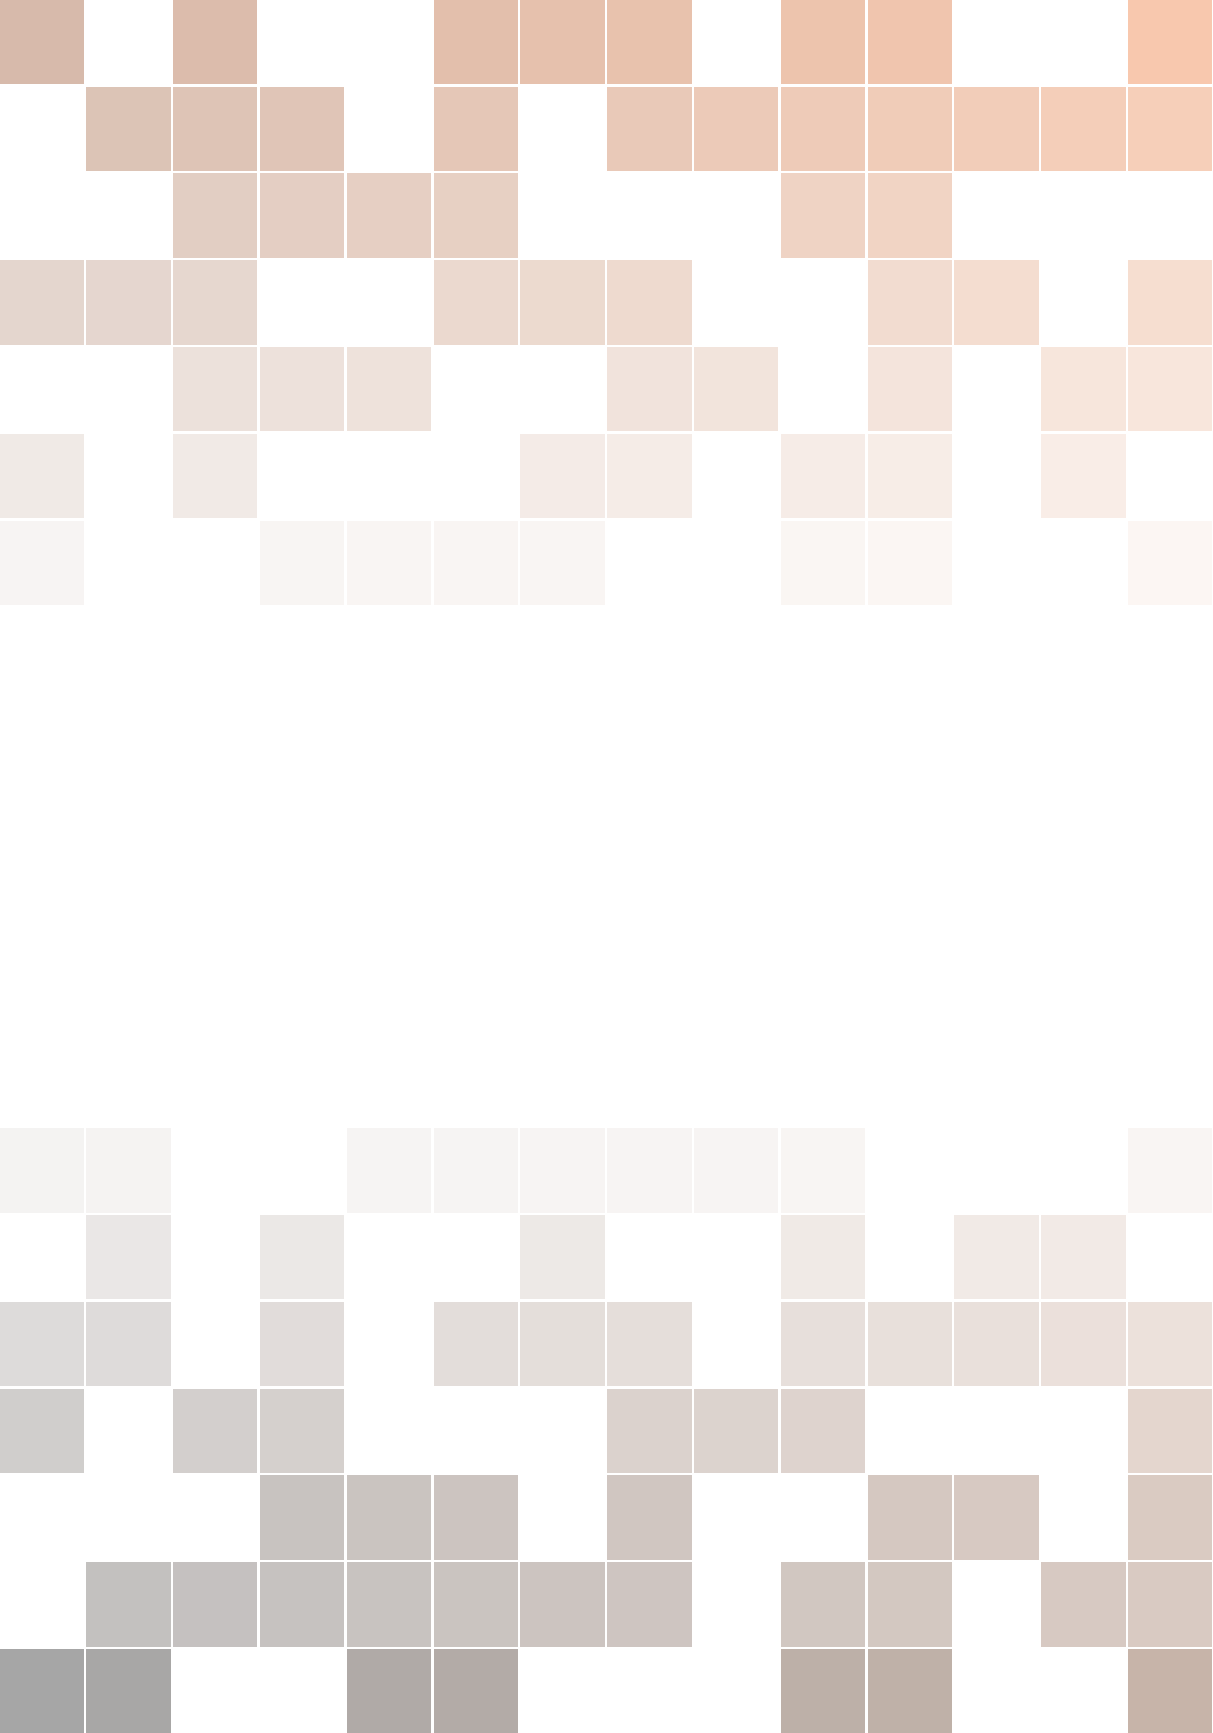
\includegraphics[scale=1]{background}}} % Image background
%\centering
%\vspace*{9cm}
%\par\normalfont\fontsize{35}{35}\sffamily\selectfont
%Mec\'anica Cl\'asica\par % Book title
%\vspace*{1cm}
%{\Huge Autores}\par % Author name
%\endgroup

%----------------------------------------------------------------------------------------
%	TABLE OF CONTENTS
%----------------------------------------------------------------------------------------
\chapterimage{Electro1} % Table of contents heading image
\pagestyle{empty} % No headers
\tableofcontents % Print the table of contents itself
\cleardoublepage % Forces the first chapter to start on an odd page so it's on the right

\pagestyle{fancy} % Print headers again


\chapter{Ecuaciones de Maxwell y propiedades din\'amicas del campo electromagn\'etico}

Las ecuaciones de Maxwell, constan de las relaciones estudiadas en cap\'itulos anteriores. Estas son:
\begin{eqnarray}
&&\nabla \times \textbf{H}=\textbf{J}, \nonumber\\
&&\nabla \times \textbf{D}=-\frac{\partial \textbf{B}}{\partial t}, \\
&&\nabla \cdot \textbf{D}=\rho, \nonumber\\
&&\nabla \cdot \textbf{B}=0.\nonumber
\end{eqnarray} \label{Ec Maxwel}
Cada una de estas expresiones representan una relaci\'on de cantidades observables experimentalmente.


%*********************SECCION********************
\section{Ley de Gauss el\'ectrico y magn\'etico para fuentes y campos variables en el tiempo}
Como hemos visto, todo el tratamiento que se ha dado es para campos y fuentes estacionaros, es decir, que no cambian en el tiempo. Ahora que pasar\'ia si se estudia el caso din\'amico.\\
Consideremos una densidad de carga volum\'etrica depende del tiempo. Si queremos calcular el campo el\'ectrico producido por esa distribuci\'on de carga en cualquier lugar del espacio, ocupamos la ley de Gauss en su forma integral.
\begin{equation}
\oint_{s} \textbf{E}(\textbf{r},t)\cdot d\textbf{s}=\frac{1}{\epsilon_{0}}\int_{V} \rho(\textbf{r},t)d \text{v}.
\end{equation}
Como el volumen de integraci\'on no depende del tiempo, entonces la dependencia temporal del campo el\'ectrico y de las fuente no afecta a la integral, por lo que se puede perfectamente el teorema de la divergencia.
\begin{eqnarray*}
\nabla\cdot\textbf{E}(\textbf{r},t)=\frac{1}{\epsilon_{0}}\rho(\textbf{r},t).
\end{eqnarray*}
Y en general, en presencia de materiales, podemos escribir la ley de Gauss en forma diferencial dependiente del tiempo como:
\begin{equation}
\therefore  \nabla\cdot\textbf{E}(\textbf{r},t)=\rho(\textbf{r},t).
\end{equation}
Podemos aplicar el mismo razonamiento para la ley de Gauss para el campo magn\'etico.\\
\begin{eqnarray*}
\oint_{s} \textbf{H}(\textbf{r})\cdot d\textbf{s}=0.
\end{eqnarray*}
Ahora suponemos que el campo magn\'etico $\textbf{H}$ y la densidad de corriente $\textbf{J}$ son funciones de la posici\'on y del tiempo.
Entonces:
\begin{eqnarray*}
\oint_{s} \textbf{H}(\textbf{r},t)\cdot d\textbf{s}=0.
\end{eqnarray*}
Por las mismas razones, la dependencia temporal no afecta a la integral, pues la regi\'on de integraci\'on no cambia con el tiempo. Aplicando el teorema de la divergencia obtenemos:
\begin{equation}
\therefore \nabla\cdot \textbf{H}(\textbf{r},t)=0.
\end{equation}


%*********************SECCION********************
\section{Ley de Faraday-Lentz-Henry}
La ley de Faraday-Henry-Lenz, establece que para toda variaci\'on del flujo que atraviesa un circuito cerrado se produce en \'este una corriente inducida. La fuerza electromotriz $\xi$ inducida en un circuito $C$ es igual a la variaci\'on del flujo \index{Flujo}  magn\'etico $\phi$ que lo atraviesa por unidad de tiempo. El sentido de la corriente inducida es tal que se opone a la variaci\'on del flujo que la produce. Estas dos afirmaciones se pueden escribir por medio de la ecuaci\'on de Faraday-Lenz que nos da el valor y el sentido de la corriente inducida.

\begin{equation}
\xi=-\frac{d \phi}{dt}.
\end{equation}\\
Aunque la ley de Faraday-Henry, a trav\'es del  signo negativo, establece una diferencia entre las corrientes inducidas por un aumento del flujo magn\'etico, no explica este fen\'omeno.\\ Lenz (1904-1965), un f\'isico alem\'an que investig\'o el electromagnetismo en Rusia al mismo tiempo que Faraday y Henry, propuso la siguiente explicaci\'on del sentido de circulaci\'on de las corrientes inducidas que se conoce como ley de Lenz:\\\\

\begin{definition}
Ley de Lenz. Las corrientes que se inducen en un circuito se producen en un sentido tal que con sus efectos magn\'eticos tienden a oponerse a la causa que las origin\'o. \cite{Wangness2001}
\end{definition}
La ley de Lenz, explica el sentido de las corrientes inducidas, puede ser a su vez explicada por un principio m\'as general, el principio de la conservaci\'on de la energ\'ia. La producci\'on de una corriente el\'ectrica requiere un consumo de energ\'ia y la acci\'on de una fuerza supone la realizaci\'on de un trabajo. En los fen\'omenos de inducci\'on electromagn\'etica es el trabajo realizado en contra de las fuerzas magn\'eticas que aparecen entre espira e im\'an el que suministra la energ\'ia necesaria para mantener la corriente inducida. Si no hay desplazamiento, el trabajo es nulo, no se transfiere energ\'ia al sistema y las corrientes inducidas no pueden aparecer.

\begin{figure}[h]
\centering
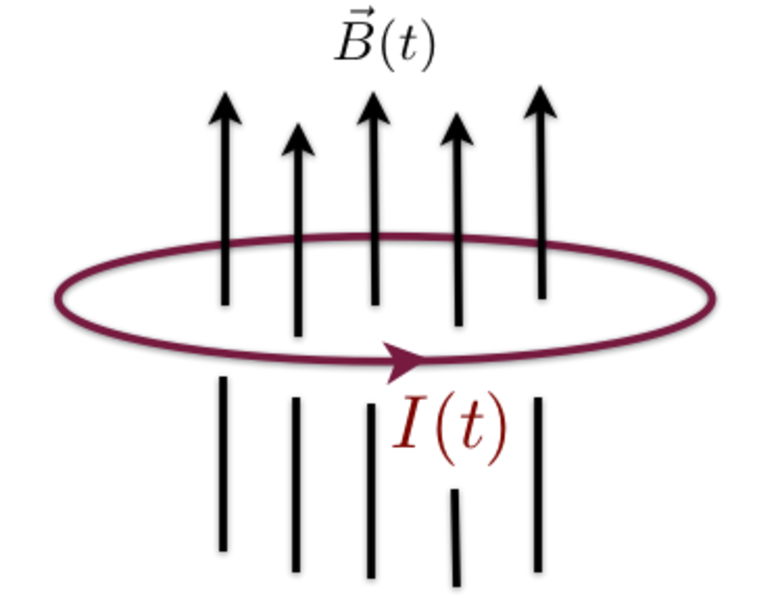
\includegraphics[width=0.45\textwidth]{Pictures/AutoIn.pdf}
\caption{Corriente inducida $I(t)$ por una variaci\'on en el campo magn\'etico $\textbf{B}(t)$}
\end{figure}

%*********************SECCION********************
\section{Conservaci\'on de la carga el\'ectrica. Corriente de desplazamiento. Ley de Amp\`ere-Maxwell}
Como indican los resultados experimentales, el principio de conservaci\'on de la carga \index{Conservacion@ Conservaci\'on ! de la carga} establece que no hay destrucci\'on ni creaci\'on neta de carga el\'ectrica, y afirma que en todo proceso electromagn\'etico la carga total de un sistema aislado se conserva. Adem\'as que la  carga el\'ectrica neta es la suma de las cargas de cada uno de sus constituyentes m\'inimos. Por ello se dice que la carga el\'ectrica est\'a cuantizada.\\\\
\subsection{Conservaci\'on de la carga el\'ectrica}
Consideremos un volumen $V$ que esta encerrado por una superficie $S$, por donde fluye una densidad de corriente $\textbf{J}$.
Entonces por la ley de Ampère:
\begin{equation}
I=\oint_{\text{s}} \textbf{J} \cdot \textbf{n} \hspace{1mm} ds.
\end{equation}
Por otro lado, como hay una densidad de corriente saliendo del volumen, esto indica que por el principio de conservaci\'on de la carga el\'ectrica, hay una disminuci\'on de ella en el volumen, esto es $-\frac{dQ}{dt}$. entonces:\\
\begin{equation}
-\frac{dQ}{dt}=\oint_{s} \textbf{J} \cdot \textbf{n}  \hspace{1mm} ds.  \label{conscarga}
\end{equation}
Adem\'as, por lo que sabemos de electrost\'atica, la carga $Q$ encerrada en el volumen $V$, se puede calcular como:\\
\begin{eqnarray*}
Q=\int_{\text{v}} \rho \, d\text{v}.
\end{eqnarray*}
sustituyendo esto ultimo en (\ref{conscarga}) obtenemos:
\begin{equation}
-\frac{d}{dt} \int_{\text{v}} \rho d\text{v}=\oint_{s} \textbf{J} \cdot \textbf{n} \hspace{1mm} ds,
\end{equation}
como el volumen $V$, no cambia en el tiempo y aplicando el teorema de la divergencia en el lado derecho de la igualdad. podemos escribir:
\begin{equation}
- \int_{\text{v}} \frac{\partial \rho}{\partial t} d\text{v}=\int_{v} \nabla \cdot \textbf{J} \hspace{1mm} d\text{v},
\end{equation}
o bien:
\begin{equation}
\int_{\text{v}} \left( \frac{\partial \rho}{\partial t} + \nabla \cdot \textbf{J} \right)   d\text{v}=0.
\end{equation}
Como esta expresi\'on es valida para cualquier volumen $V$, entonces el integrando es valido para cualquier punto, la cual se conoce como ecuaci\'on de continuidad. \index{Ecuacion@Ecuaci\'on ! de continuidad} \cite{Griffiths1999}
\begin{equation}
 \frac{\partial \rho}{\partial t} + \nabla \cdot \textbf{J}=0.  \label{continuidad}
 \end{equation}

\subsection{Corriente de desplazamiento y Ley de Amp\`ere-Maxwell}

Como ya se ha visto, el campo magn\'etico debido a una distribuci\'on de corriente obedece a la ley de Ampère:
\begin{equation}
\nabla \times \textbf{H}= \textbf{J}. \label{ecampere}
\end{equation}
Adem\'as es bien sabido que para cualquier vector $\textbf{A}$, la divergencia del rotacional de $\textbf{A}$ es siempre cero. revisemos que pasa con la ley de Ampère:
\begin{eqnarray*}
\nabla \cdot(\nabla \times \textbf{H})=\nabla \cdot \textbf{J}.
\end{eqnarray*}
Por otro lado, sustituyendo la expresi\'on (\ref{continuidad}) en la anterior.
\begin{equation}
\nabla \cdot(\nabla \times \textbf{H})=-\frac{\partial \rho}{\partial t}. \label{divrotH}
\end{equation}
Como $-\frac{\partial \rho}{\partial t}$ en general no es siempre cero; es claro que la ecuaci\'on (\ref{ecampere}) necesita una modificaci\'on.
Para arreglar esta problema, Maxwell supuso que esta ecuaci\'on estaba incompleta, por lo que el propuso esta expresi\'on.
\begin{equation}
\nabla \times \textbf{H}= \textbf{J}+\textbf{J}_{d}.  \label{amperemod}
\end{equation}
Con $\textbf{J}_{d}$ un termino adicional que se necesita hallar.\
Al sustituir la expresi\'on (\ref{amperemod}) en (\ref{divrotH}):
\begin{eqnarray*}
\nabla \cdot(\nabla \times \textbf{H})=\nabla \cdot \textbf{J}+\nabla \cdot \textbf{J}_{d},
\end{eqnarray*}
\begin{eqnarray*}
\nabla \cdot(\nabla \times \textbf{H})=-\frac{\partial \rho}{\partial t}+\nabla \cdot \textbf{J}_{d}.
\end{eqnarray*}

Por otro lado, sabemos que podemos expresar a la densidad de carga $\rho$ en t\'erminos del vector de desplazamiento $\textbf{D}$.
\begin{eqnarray*}
\nabla \cdot(\nabla \times \textbf{H})=-\frac{\partial}{\partial t} \nabla \cdot \textbf{D} +\nabla \cdot \textbf{J}_{d}.
\end{eqnarray*}

Como $\nabla \cdot(\nabla \times \textbf{H})=0$, entonces si suponemos que $\textbf{D}$ es una funci\'on bien comportada, se puede intercambiar el orden de las derivadas parciales, obteniendo:
\begin{equation}
\nabla \cdot \left( \textbf{J}_{d}-\frac{\partial \textbf{D}}{\partial t} \right)=0.
\end{equation}
De aqu\'i se puede ver que $\textbf{J}_{d}-\frac{\partial \textbf{D}}{\partial t}=\textbf{0}$, es decir,
\begin{equation}
\textbf{J}_{d}=\frac{\partial \textbf{D}}{\partial t}.
\end{equation}
De modo que, ahora la ecuaci\'on de Ampère se transforma en:
\begin{equation}
\nabla \times \textbf{H}= \textbf{J}+\frac{\partial \textbf{D}}{\partial t}. \label{AmpereMaxwell}
\end{equation}
Esta expresi\'on se conoce como la ley de Amp\`ere-Maxwell y el termino $\textbf{J}_{d}$ se le dio el nombre de corriente de desplazamiento.\index{Corriente de desplazamiento }\cite{Milford1986} \\
Como se ha modificado la forma de $\nabla \times \textbf{H}$, es conveniente ver como han cambiado algunos de los resultados obtenidos anteriormente. Por ejemplo la forma integral de la ley de Ampère.

%***** Observación****************

\begin{obs}
Podemos tomar la expresi\'on (\ref{AmpereMaxwell}) en su forma integral y aplicar el teorema de Stokes,
\begin{eqnarray*}
\int_{S} \nabla \times \textbf{H} \cdot d\textbf{s}=\oint_{C} \textbf{H}\cdot d\textbf{s},
\end{eqnarray*}
\begin{eqnarray*}
\int_{S} \nabla \times \textbf{H} \cdot d\textbf{s}=\oint_{C} (\textbf{J}_{f}+\textbf{J}_{d})\cdot d\textbf{s},
\end{eqnarray*}
\begin{eqnarray*}
\int_{S} \nabla \times \textbf{H} \cdot d\textbf{s}=\oint_{C} \textbf{J}_{f}\cdot d\textbf{s}+\oint_{C}\frac{\partial \textbf{D}}{\partial t}\cdot d\textbf{s},
\end{eqnarray*}
\begin{equation}
\oint_{C} \textbf{H}\cdot d\textbf{s}=I_{f}+I_{d}.  \label{SumdecorrientesAmpere}
\end{equation}
Donde $I_{f}$ y $I_{d}$ son corriente de cargas libres y corriente de desplazamiento respectivamente. Cuando $\textbf{D}$ es constante en el tiempo, se regresa a la ley de Ampère.\\\\
\end{obs}


%*********************EJEMPLO********************
\begin{example}
 Se tiene un capacitor de placas paralelas circulares en proceso de carga, con radio $a$, se supone que existe un vac\'io entre las placas y se supone que la separaci\'on entre ellas es tan pequeña comparada con el radio, que se puede suponer que el campo el\'ectrico $\textbf{E}$ es uniforme y esta confinado enteramente entre las placas. Encontrar el campo $\textbf{H}$ en todo el espacio.\\
\begin{figure}[hbtp]
\centering
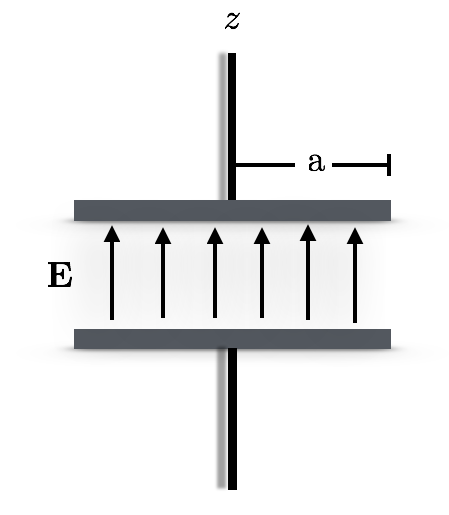
\includegraphics[scale=0.25]{Pictures/condensadorcircular.png}
\caption{\text{ Condensador circular}}
\end{figure}
%********************** Solucion*************************
\emph{Soluci\'on.}\\

Para encontrar el campo magn\'etico $\textbf{H}$, ocuparemos la ecuaci\'on (\ref{AmpereMaxwell}), de tal modo que necesitamos calcular primero las densidades de corriente $\textbf{J}_{f}$ y $\textbf{J}_{d}$.\\
Por otro lado el vector desplazamiento $\textbf{D}$ en el vac\'io esta definido como:\\
\begin{equation}
\textbf{D}=\epsilon_{0} \textbf{E}.
\end{equation}

Como sabemos,el campo el\'ectrico $\textbf{E}$ entre las placas de capacitor esta dado por $\textbf{E}=\frac{\sigma_{f}}{\epsilon_{0}}\hat{\textbf{z}}$, en funci\'on de la densidad de carga libre $\sigma_{f}$, esto sucede en el caso electrost\'atico, en que la carga tiene un valor constante y se encuentra uniformemente distribuida sobre la superficie de la placa. Pero el problema supone que el capacitor se esta cargando por medio de una corriente constante $\frac{dq}{dt}$, esto es logra introduciendo una corriente $I=\frac{dq}{dt}$ que pasa por un alambre en sobre el eje $z$\\
Para que se siga conservando una densidad de carga superficial uniformemente distribuida se tiene que suponer que la carga adquirida se distribuye instant\'aneamente sobre la superficie de la placa. \\
Por otro lado el vector desplazamiento $\textbf{D}$ en el vac\'io esta definido como:\\
\begin{eqnarray*}
\textbf{D}=\epsilon_{0} \textbf{E},
\end{eqnarray*}
\begin{eqnarray*}
\textbf{D}=\epsilon_{0} \textbf{E}=\frac{q}{\pi a^{2} }\hat{\textbf{z}},
\end{eqnarray*}
en t\'erminos de la carga total $q$ y la superficie de la placa $\pi a^{2}$. Por lo tanto la densidad de corriente $\textbf{J}_{d}$ se puede calcular como:
\begin{eqnarray*}
\textbf{J}_{d}=\frac{\partial \textbf{D}}{\partial t} \hat{\textbf{z}}.
\end{eqnarray*}
Dado que $q$ no es constante, pues el capacitor se esta cargando por medio de una corriente $I$, entonces:\\
\begin{eqnarray*}
\textbf{J}_{d}=\frac{1}{\pi a^{2}}\frac{dq}{dt} \hat{\textbf{z}},
\end{eqnarray*}
\begin{equation}
\textbf{J}_{d}=\frac{I}{\pi a^{2}} \hat{\textbf{z}}. \label{Jdesplazamiento}
\end{equation}
Sabiendo que la corriente de desplazamiento que atraviesa una superficie $S$ es:
\begin{eqnarray*}
I_{d}=\int_{S} \textbf{J}_{d} \cdot d\textbf{s}.
\end{eqnarray*}
Sustituyendo la expresi\'on (\ref{Jdesplazamiento}) obtenemos,
\begin{eqnarray*}
I_{d}=\int_{S} \frac{I}{\pi a^{2}} \hat{\textbf{z}} \cdot d\textbf{s}=I.
\end{eqnarray*}
Que es la corriente total que aporta la carga del capacitor. Como las placas son circulares y la corriente pasa por el eje $z$, podemos concluir que $\textbf{H}$, tiene simetr\'ia axial con el eje $z$, por lo tanto podemos pensar en $\textbf{H}$ de la forma $ \textbf{H}=H_{\varphi}(\rho)\hat{\varphi}$, entonces:\\
\begin{eqnarray*}
\oint_{C} \textbf{H} \cdot d\textbf{s}=\oint_{C} H_{\varphi}(\rho)\hat{\varphi} \cdot d\textbf{s}.
\end{eqnarray*}
Integrando en una trayectoria circular $C$, con radio $\rho$ y centro en el eje $z$ perpendicular a este:
\begin{eqnarray*}
\oint_{C} \textbf{H} \cdot d\textbf{s}=H_{\varphi} 2 \pi \rho.
\end{eqnarray*}
Por lo tanto de acuerdo a la ecuaci\'on (\ref{SumdecorrientesAmpere}), podemos despejar $H_{\varphi}$ como:
\begin{equation}
H_{\varphi}(\rho)=\frac{I_{f}+I_{d}}{2 \pi \rho}.
\end{equation}
Resulta conveniente dividir el espacio en 4 regiones, las regiones $3$ y $4$ fuera del condensador, vemos que $I_{f}=I$, mientras que $I_{d}=0$, con lo que se obtiene:
\begin{eqnarray*}
H_{\varphi 3}(\rho)=H_{\varphi 4}(\rho)=\frac{I}{2 \pi \rho}.
\end{eqnarray*}
Para la regi\'on 2 $(\rho>a)$, se utiliza una trayectoria de integraci\'on $C$ con $\rho>a$, entonces $I_{f}=0$ y $I_{d}=I$. obteniendo:
\begin{equation}
H_{\varphi 2}(\rho)=\frac{I}{2 \pi \rho}  \hspace{2cm} (\rho>a).
\end{equation}
Finalmente para la regi\'on $1$, donde $\rho<a$, tenemos que $I_{f}=0$ y $I_{d}=I\frac{\rho^{2}}{a^{2}}$, por lo tanto, el campo $\textbf{H}$ para esta regi\'on es:
\begin{equation}
H_{\varphi 2}(\rho)=\frac{I\rho}{2 \pi a^{2}}  \hspace{2cm} (\rho<a).
\end{equation}
\end{example}


%*********************EJEMPLO********************
\begin{example}
Un capacitor de placas paralelas consiste de dos placas circulares de \'area S con un vac\'io entre ellas. Se conectan a una bater\'ia de \emph{fem} constante. Se hacen oscilar lentamente de modo que sigan siendo paralelas pero la separaci\'on $d$ cambie seg\'un $d=d_{0}+d_{1}\sen\omega t$. Encontrar el campo magn\'etico $\textbf{H}$ que se produce entre las dos placas por la corriente de desplazamiento. De manera similar, encontrar $\textbf{H}$ si primero se desconecta el capacitor de la bater\'ia y despu\'es se hace que las placas oscilen de la misma manera.
\begin{figure}[hbtp]
\centering
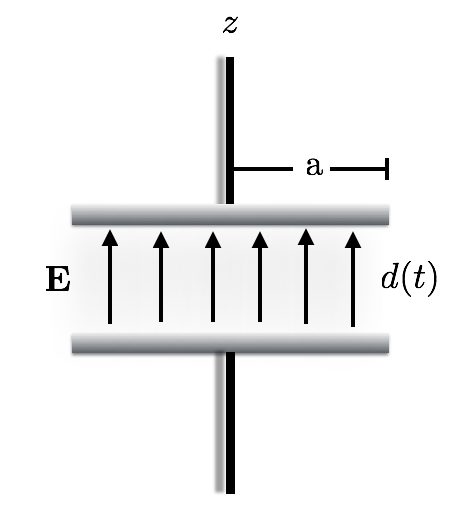
\includegraphics[scale=0.50]{Pictures/ConVariablet.png}
\caption{Capacitor que oscila lentamente}
\end{figure}

\emph{Soluci\'on.}\\
%*************** Solucion*************************
Podemos calcular el campo el\'ectrico entre las placas de un capacitor con una diferencia de potencial $V$ y la distancia entre las placas $d$ ya que la variaci\'on de la distancia es muy lenta y podemos considerar al campo el\'ectrico uniforme.
\begin{eqnarray*}
\textbf{E}=\frac{V}{d} \hspace{1mm} \hat{\textbf{n}}
\end{eqnarray*}
Para el problema, tenemos el circuito alimentado por una bater\'ia de una \emph{fem} constante, es decir, una diferencia de potencial de $\xi_{0}$. Entonces para el campo el\'ectrico del capacitor es:
\begin{equation}
\textbf{E}=\frac{\xi_{0}}{d_{0}+d_{1}\sen\omega t}\hspace{1mm} \hat{\textbf{n}}.
\end{equation}
Por otro lado, como hay un vac\'io entre las placas, no hay cargas libres en el capacitor. Por lo tanto, no hay densidades de corriente $\textbf{J}_{f}$:\\
Necesitamos calcular la densidad de corriente de desplazamiento $J_{d}$, esto es $\frac{\partial \textbf{D}}{\partial t}$,adem\'as sabemos que $\textbf{D}=\epsilon_{0}\textbf{E}$. Entonces:\\
\begin{equation}
\textbf{J}_{d}=\epsilon_{0}\frac{\partial \textbf{E}}{\partial t},
\end{equation}
\begin{eqnarray*}
\textbf{J}_{d}=\epsilon_{0}\frac{\partial}{\partial t} \left( \frac{\xi_{0}}{d_{0}+d_{1}\sen
\omega t}\hspace{1mm} \hat{\textbf{z}} \right),
\end{eqnarray*}
\begin{equation}
\textbf{J}_{d}=-\frac{\epsilon_{0}\xi_{0}\omega d_{1} \hspace{1mm} \cos \omega t }{(d_{0}+d_{1}\sen\omega t)^{2}}  \hat{\textbf{z}}.
\end{equation}
Calculando la corriente de desplazamiento $I_{d}$ que atraviesa una superficie circular $S$ que pasa por el eje $z$ aprovechando la simetr\'ia axial.
\begin{equation}
I_{d}=\int_{S} \textbf{J}_{d} \cdot d\textbf{s}.
\end{equation}
\begin{eqnarray*}
I_{d}=-\int_{0}^{\rho} \int_{0}^{2\pi} \frac{\epsilon_{0}\xi_{0}\omega d_{1} \hspace{1mm} \cos \omega t }{(d_{0}+d_{1}\sen\omega t)^{2}}  \rho^{'} d\rho^{'} d\theta^{'},
\end{eqnarray*}
\begin{equation}
I_{d}=-\frac{\pi\rho^{2} \epsilon_{0}\xi_{0}\omega d_{1} \hspace{1mm} \cos \omega t }{(d_{0}+d_{1}\sen\omega t)^{2}}.
\end{equation}
Entonces usando la expresi\'on (\ref{SumdecorrientesAmpere}) para calcular el campo $\textbf{H}$:
\begin{eqnarray*}
\oint_{c} \textbf{H} \cdot d\textbf{s}=I_{f}+I_{d}.
\end{eqnarray*}
Donde $C$ es la curva que encierra la superficie $S$, de modo que usando la simetr\'ia axial del eje $z$ la integral se transforma en:
\begin{eqnarray*}
\oint_{c} H_{\varphi} ds=I_{d},
\end{eqnarray*}
\begin{eqnarray*}
H_{\varphi} 2\pi\varphi=I_{d}.
\end{eqnarray*}
Sustituyendo la corriente de desplazamiento en la expresi\'on anterior
\begin{equation}
H_{\varphi} 2\pi\varphi=-\frac{\pi\rho^{2} \epsilon_{0}\xi_{0}\omega d_{1} \hspace{1mm} \cos \omega t }{(d_{0}+d_{1}\sen\omega t)^{2}}.
\end{equation}
De modo que:
\begin{equation}
H_{\varphi} =-\frac{\rho \epsilon_{0}\xi_{0}\omega d_{1} \hspace{1mm} \cos \omega t }{2(d_{0}+d_{1}\sen\omega t)^{2}}.
\end{equation}
Por lo tanto, el campo $\textbf{H}$ en funci\'on de $\rho$ esta dado por:
\begin{equation}
H_{\varphi} (\rho) =-\frac{\rho \epsilon_{0}\xi_{0}\omega d_{1} \hspace{1mm} \cos \omega t }{2(d_{0}+d_{1}\sen\omega t)^{2}}.
\end{equation}
\end{example}

%*********************SECCION********************
\section{Modificaciones en presencia de medios diel\'ectricos y permeables, y de conductores}
Despu\'es de agregar la correcci\'on de  Maxwell a la ecuaci\'on de Ampère, se puede llegar a un conocimiento completo del electromagnetismo resumido por medio de cuatro ecuaciones vectoriales:\\
\begin{equation}
\nabla \cdot \textbf{D}=\rho, \label{GaussElect}
 \end{equation}
 \begin{equation}
 \nabla \times \textbf{E}=-\frac{\partial \textbf{B}}{\partial t},  \label{Faraday}
 \end{equation}
 \begin{equation}
 \nabla \cdot \textbf{B}=0,  \label{GaussMagn}
 \end{equation}
 \begin{equation}
 \nabla \times \textbf{H}=\textbf{J}+\frac{\partial \textbf{D}}{\partial t}.  \label{DesplaAmpereMaxwell}
 \end{equation}
 Estas ecuaciones son conocidas como las ecuaciones de Maxwell y describen cualquier fen\'omeno electromagn\'etico. Vale la pena repasar un poco el contenido f\'isico de estas ecuaciones:\\\\
 La ecuaci\'on (\ref{GaussElect}) resume la ley de Coulomb, es decir, la fuerza entre cargas el\'ectricas tomando en cuenta los efectos el\'ectricos de la materia. La ecuaci\'on (\ref{Faraday}) representa la ley de inducci\'on de Faraday y relaciona los campos el\'ectricos y magn\'eticos. Mientras que la ecuaci\'on (\ref{GaussMagn}) es una forma de recordar el hecho que no existen cargas magn\'eticas libres, siempre se encuentran en pares. La ultima ecuaci\'on (\ref{DesplaAmpereMaxwell}) incluye la ley de Ampère para la interacci\'on entre corrientes el\'ectricas y los efectos magn\'eticos de la materia.\\
Es conveniente recordar que estas ecuaciones se tienen que complementar con otras relaciones que involucran la descripci\'on electromagn\'etica de la materia.
\begin{equation}
\textbf{D}=\epsilon_{0} \textbf{E}+\textbf{P},  \label{VectorDesplazamineto}
\end{equation}
\begin{equation}
\textbf{H}=\frac{\textbf{B}}{\mu_{0}}-\textbf{M}.  \label{Campo H}
\end{equation}
Reescribiendo las ecuaciones de Maxwell con las expresiones (\ref{VectorDesplazamineto}) y (\ref{Campo H}).
\begin{equation}
\nabla \cdot \textbf{E}=\frac{1}{\epsilon_{0}}(\rho-\nabla\cdot\textbf{P}), \label{GaussElectcargaslibres}
 \end{equation}
 \begin{equation}
 \nabla \times \textbf{E}=-\frac{\partial \textbf{B}}{\partial t},
 \end{equation}
 \begin{equation}
 \nabla \cdot \textbf{B}=0,
 \end{equation}
 \begin{equation}
\nabla \times \textbf{B}=\mu_{0}\left( \textbf{J}+\nabla \times \textbf{M}+\epsilon_{0}\frac{\partial \textbf{E}}{\partial t}+\frac{\partial \textbf{P}}{\partial t}\right). \label{AmpereMaxwelMagnetizacion}
 \end{equation}
Dos de estas ecuaciones cambiaron, su forma ya no es tan compacta. Sin embargo, resultan f\'acilmente comprensibles: el termino entre par\'entesis de la ecuaci\'on (\ref{GaussElectcargaslibres}) es la densidad total de carga, escrita como la suma de de la densidad de carga libre mas la densidad de carga ligada. De forma an\'aloga el termino entre par\'entesis de la ecuaci\'on (\ref{AmpereMaxwelMagnetizacion}) representa la densidad total de corriente, los dos primeros t\'erminos corresponden a la densidad de corriente libre y a la densidad de corriente de magnetizaci\'on, los otros dos t\'erminos corresponden a la densidad de corriente de desplazamiento del vac\'io y la de densidad de corriente de polarizaci\'on  asociada a las cargas ligadas en movimiento.\\\\
Una situaci\'on especial, se da cuando se trabaja con medios isotr\'opicos homog\'eneos lineales. En estos casos, el campo magn\'etico $\textbf{B}$, el vector desplazamiento $\textbf{D}$ y la densidad de corriente libre $\textbf{J}$ se pueden expresar como:\
\begin{equation}
\textbf{D}=\epsilon\textbf{E},
\end{equation}
\begin{equation}
\textbf{B}=\mu \textbf{H},
\end{equation}
\begin{equation}
\textbf{J}=\sigma\textbf{E}+\textbf{J}^{'}.
\end{equation}
Donde $\epsilon,\mu,\sigma$ son constantes caracter\'isticas de los materiales y $\textbf{J}^{'}$ es una densidad de corriente libre proveniente de otras fuentes.
Entonces las ecuaciones:
\begin{eqnarray*}
\nabla \cdot \textbf{D}=\rho,
 \end{eqnarray*}
 \begin{eqnarray*}
 \nabla \times \textbf{E}=-\frac{\partial \textbf{B}}{\partial t},
 \end{eqnarray*}
 \begin{eqnarray*}
 \nabla \cdot \textbf{B}=0,
 \end{eqnarray*}
 \begin{eqnarray*}
 \nabla \times \textbf{H}=\textbf{J}+\frac{\partial \textbf{D}}{\partial t}.
 \end{eqnarray*}
 se pueden reescribir como:
 \begin{equation}
\nabla\cdot \textbf{E}=\frac{\rho}{\epsilon},
 \end{equation}
\begin{equation}
\nabla \times \textbf{E}=-\frac{\partial \textbf{B}}{\partial t},
\end{equation}
\begin{equation}
\nabla \cdot \textbf{B}=0,
\end{equation}
\begin{equation}
\nabla \times \textbf{B}=\mu\sigma\textbf{E}+\mu\textbf{J}^{'}+\mu\epsilon\frac{\partial \textbf{E}}{\partial t}. \label{AmpereMateria}
\end{equation}

%*********************SECCION********************
\section{Potencial vectorial y escalar. Transformaci\'on de la norma}
\subsection{Potencial vectorial y escalar}
Como se estudio en secciones anteriores, el estudio de cualquier fen\'omeno electromagn\'etico esta descrito por las ecuaciones de Maxwell.
\begin{equation}
\nabla \cdot \textbf{E}=\frac{1}{\epsilon_{0}}(\rho-\nabla\cdot\textbf{P}),
 \end{equation}
 \begin{equation}
 \nabla \times \textbf{E}=-\frac{\partial \textbf{B}}{\partial t},
 \end{equation}
 \begin{equation}
 \nabla \cdot \textbf{B}=0,
 \end{equation}
 \begin{equation}
\nabla \times \textbf{B}=\mu_{0}\left( \textbf{J}+\nabla \times \textbf{M}+\epsilon_{0}\frac{\partial \textbf{E}}{\partial t}+\frac{\partial \textbf{P}}{\partial t}\right).
 \end{equation}
Como podemos ver, la expresi\'on de la ley de Gauss para el campo magn\'etico, $\nabla \cdot \textbf{B}=0$, fue usada para definir el potencial vectorial magn\'etico $\textbf{A}$.
\begin{equation}
 \textbf{B}(\textbf{r},t)=\nabla \times \textbf{A}(\textbf{r},t),  \label{VectorA}
 \end{equation}
 ya que para cualquier vector $\textbf{C}$ siempre se tiene que cumplir la identidad
 \begin{eqnarray*}
 \nabla \cdot(\nabla \times \textbf{C})=0.
 \end{eqnarray*}
 Si se sustituye la expresi\'on (\ref{VectorA}) en (\ref{Faraday}), tenemos:
 \begin{eqnarray*}
 \nabla \times \textbf{E}=-\frac{\partial \textbf{B}}{\partial t},
 \end{eqnarray*}
 \begin{eqnarray*}
 \nabla \times \textbf{E}=-\frac{\partial}{\partial t}\left( \nabla  \times \textbf{A} \right),
 \end{eqnarray*}
 \begin{eqnarray*}
 \nabla \times \textbf{E}=-\nabla \times \frac{\partial \textbf{A}}{\partial t},
 \end{eqnarray*}
  \begin{equation}
\nabla \times \left( \textbf{E}+\frac{\partial \textbf{A}}{\partial t} \right)=0. \label{potencial}
  \end{equation}
Por otro lado, recordando la identidad vectorial $\nabla \times \textbf{C}=\textbf{0}$ de modo que $\textbf{C}=-\nabla V$, es decir, el rotacional del gradiente de una funci\'on escalar $V$ siempre es cero. Por lo tanto se puede reescribir el termino entre par\'entesis de la ecuaci\'on (\ref{potencial}) como:
\begin{eqnarray*}
-\nabla \phi=\textbf{E}+\frac{\partial \textbf{A}}{\partial t}.
\end{eqnarray*}
Entonces tenemos una expresi\'on general para el campo el\'ectrico $\textbf{E}$:
\begin{equation}
\textbf{E}=-\nabla \phi-\frac{\partial \textbf{A}}{\partial t}.  \label{CampoEcompleto}
\end{equation}
Al sustituir la expresi\'on  (\ref{CampoEcompleto}) en (\ref{GaussElectcargaslibres}) tenemos:
\begin{eqnarray*}
\nabla \cdot \textbf{E}=\frac{1}{\epsilon_{0}}\left(\rho-\nabla \cdot \textbf{P}\right),
\end{eqnarray*}
\begin{eqnarray*}
\nabla \cdot \left(-\nabla \phi-\frac{\partial \textbf{A}}{\partial t}\right) =\frac{1}{\epsilon_{0}}\left(\rho-\nabla \cdot \textbf{P}\right),
\end{eqnarray*}
\begin{equation}
-\nabla^{2}\phi -\frac{\partial}{\partial t}\left(\nabla \cdot \textbf{A}\right)  =\frac{1}{\epsilon_{0}}\left(\rho-\nabla \cdot \textbf{P}\right).  \label{EcuacionPotencial}
\end{equation}
An\'alogamente al sustituir las ecuaciones (\ref{VectorA}) y (\ref{CampoEcompleto}) en (\ref{AmpereMaxwelMagnetizacion}), obtenemos:
\begin{eqnarray*}
\nabla \times \textbf{B}=\mu_{0}\left[\textbf{J}+\nabla \times \textbf{M}+\epsilon_{0}\frac{\partial \textbf{E}}{\partial t}+\frac{\partial \textbf{P}}{\partial t} \right],
\end{eqnarray*}
\begin{eqnarray*}
\nabla \times (\nabla \times \textbf{A})=\mu_{0}\left[\textbf{J}+\nabla \times \textbf{M}+\epsilon_{0}\frac{\partial}{\partial t} \left( -\nabla \phi-\frac{\partial \textbf{A}}{\partial t} \right)  +\frac{\partial \textbf{P}}{\partial t} \right],
\end{eqnarray*}
\begin{eqnarray*}
\nabla(\nabla \cdot \textbf{A})-\nabla^{2} \textbf{A}=\mu_{0}\left[\textbf{J}+\nabla \times \textbf{M}+\epsilon_{0}\left(-\nabla\frac{\partial \phi}{\partial t}-\frac{\partial^{2} \textbf{A}}{\partial t^{2}} \right)  +\frac{\partial \textbf{P}}{\partial t} \right],
\end{eqnarray*}
\begin{eqnarray*}
\nabla(\nabla \cdot \textbf{A})-\nabla^{2} \textbf{A}=-\epsilon_{0}\mu_{0}\nabla\frac{\partial \phi}{\partial t}+\mu_{0}\left[\textbf{J}+\nabla \times \textbf{M}-\epsilon_{0}\frac{\partial^{2} \textbf{A}}{\partial t^{2}} +\frac{\partial \textbf{P}}{\partial t} \right],
\end{eqnarray*}
\begin{eqnarray*}
\nabla(\nabla \cdot \textbf{A})+\epsilon_{0}\mu_{0}\nabla\frac{\partial \phi}{\partial t}-\nabla^{2} \textbf{A}+\epsilon_{0}\mu_{0}\frac{\partial^{2} \textbf{A}}{\partial t^{2}}=\mu_{0}\left[\textbf{J}+\nabla \times \textbf{M} +\frac{\partial \textbf{P}}{\partial t} \right],
\end{eqnarray*}
\begin{equation}
\nabla\left(\nabla \cdot \textbf{A}+\epsilon_{0}\mu_{0}\frac{\partial \phi}{\partial t}\right)-\nabla^{2} \textbf{A}+\epsilon_{0}\mu_{0}\frac{\partial^{2} \textbf{A}}{\partial t^{2}}=\mu_{0}\left[\textbf{J}+\nabla \times \textbf{M}+\frac{\partial \textbf{P}}{\partial t} \right].  \label{EcuacionA}
\end{equation}
Gracias a estas sustituciones se obtuvieron dos ecuaciones diferenciales para $\textbf{A}$ y $\phi$, de modo que encontrando su soluci\'on, autom\'aticamente, se tienes todos las campos $\textbf{E}$ y $\textbf{B}$ que satisfacen las ecuaciones de Maxwell.\cite{Wangness2001} \\\\
Un caso especial se da cuando se trabaja en materiales isotr\'opicos homog\'eneos lineales, entonces utilizando las expresiones de las ecuaciones de Maxwell para estos medios, estudiados en la secci\'on anterior, sustituyendo la expresi\'on general para el campo el\'ectrico en la divergencia de $\textbf{E}$, tenemos:
\begin{eqnarray*}
\nabla\cdot\textbf{E}=\frac{\rho}{\epsilon},
\end{eqnarray*}
\begin{eqnarray*}
\nabla\cdot\left(-\nabla\phi-\frac{\partial \textbf{A}}{\partial t}\right)=\frac{\rho}{\epsilon},
\end{eqnarray*}
\begin{equation}
\nabla^{2}\phi+\nabla\cdot\frac{\partial \textbf{A}}{\partial t}=-\frac{\rho}{\epsilon}. \label{Ec. potencial}
\end{equation}
Ahora si sustituimos las expresiones (\ref{VectorA}) y (\ref{CampoEcompleto}) en la ecuaci\'on (\ref{AmpereMateria}):
\begin{eqnarray*}
\nabla \times \textbf{B}=\mu\sigma\textbf{E}+\mu\textbf{J}^{'}+\mu\epsilon\frac{\partial \textbf{E}}{\partial t},
\end{eqnarray*}
\begin{eqnarray*}
\nabla \times (\nabla\times\textbf{A})=\mu\sigma\left(-\nabla\phi-\frac{\partial \textbf{A}}{\partial t}\right)+\mu\textbf{J}^{'}+\mu\epsilon\frac{\partial}{\partial t} \left(-\nabla\phi-\frac{\partial \textbf{A}}{\partial t}\right).
\end{eqnarray*}
Usando la identidad $\nabla\times\textbf{C}=\nabla(\nabla\cdot\textbf{A})-\nabla^{2}\textbf{C}$ y realizando las derivadas respecto al tiempo:
\begin{eqnarray*}
\nabla(\nabla\cdot\textbf{A})-\nabla^{2}\textbf{A}=-\mu\sigma\nabla\phi-\mu\sigma\frac{\partial \textbf{A}}{\partial t}+\mu\textbf{J}^{'}-\mu\epsilon\nabla\frac{\partial \phi}{\partial t}-\mu\epsilon\frac{\partial^{2} \textbf{A}}{\partial t^{2}}.
\end{eqnarray*}
 Agrupando t\'erminos:
\begin{eqnarray*}
\nabla(\nabla\cdot\textbf{A})-\nabla^{2}\textbf{A}=-\nabla\left(\mu\sigma\phi-\mu\epsilon\frac{\partial \phi}{\partial t}\right)-\mu\epsilon\frac{\partial^{2} \textbf{A}}{\partial t^{2}}-\mu\sigma\frac{\partial \textbf{A}}{\partial t}+\textbf{J}^{'},
\end{eqnarray*}
\begin{equation}
\nabla^{2}\textbf{A}-\mu\sigma\frac{\partial \textbf{A}}{\partial t}-\mu\epsilon\frac{\partial^{2} \textbf{A}}{\partial t^{2}}-\nabla\left(\nabla\cdot\textbf{A}+\mu\sigma\phi+\mu\epsilon\frac{\partial \phi}{\partial t}\right)=-\mu\textbf{J}^{'}. \label{EcuacionAmateria}
\end{equation}
Si sumamos y restamos los t\'erminos $-\mu\sigma\frac{\partial \phi}{\partial t}-\mu\epsilon\frac{\partial^{2} \phi}{\partial t^{2}}$ a la ecuaci\'on (\ref{Ec. potencial}), podemos obtener una expresi\'on similar a la ecuaci\'on (\ref{EcuacionAmateria})
\begin{eqnarray*}
\nabla^{2}\phi+\nabla\cdot\frac{\partial \textbf{A}}{\partial t}=-\frac{\rho}{\epsilon},
\end{eqnarray*}
\begin{eqnarray*}
\nabla^{2}\phi+\nabla\cdot\frac{\partial \textbf{A}}{\partial t}-\mu\sigma\frac{\partial \phi}{\partial t}-\mu\epsilon\frac{\partial^{2} \phi}{\partial t^{2}}+\mu\sigma\frac{\partial \phi}{\partial t}+\mu\epsilon\frac{\partial^{2} \phi}{\partial t^{2}}=-\frac{\rho}{\epsilon}.
\end{eqnarray*}
reordenando y agrupando t\'erminos, obtenemos:
\begin{equation}
\nabla^{2}\phi-\mu\sigma\frac{\partial \phi}{\partial t}-\mu\epsilon\frac{\partial^{2} \phi}{\partial t^{2}}+\frac{\partial}{\partial t}\left(\nabla\cdot\textbf{A}+\mu\sigma\phi+\mu\epsilon\frac{\partial \phi}{\partial t}\right)=-\frac{\rho}{\epsilon}. \label{Ec. Potencial materia}
\end{equation}
Al comparar las ecuaciones (\ref{EcuacionAmateria}) y (\ref{Ec. Potencial materia}) podemos ver que si el factor
\begin{equation}
\nabla\cdot\textbf{A}+\mu\sigma\phi+\mu\epsilon\frac{\partial \phi}{\partial t}=0.  \label{CondiciondeLorentz}
\end{equation}
Entonces obtenemos las ecuaciones:
\begin{equation}
\nabla^{2}\textbf{A}-\mu\sigma\frac{\partial \textbf{A}}{\partial t}-\mu\epsilon\frac{\partial^{2} \textbf{A}}{\partial t^{2}}=-\mu\textbf{J}^{'},
\end{equation}
\begin{equation}
\nabla^{2}\phi-\mu\sigma\frac{\partial \phi}{\partial t}-\mu\epsilon\frac{\partial^{2} \phi}{\partial t^{2}}=-\frac{\rho}{\epsilon}.
\end{equation}
A la expresi\'on (\ref{CondiciondeLorentz}) se le conoce como condici\'on de Lorentz. Esta condici\'on nos proporciona ecuaciones para $\textbf{A}$ y $\phi$ independientes entre si; adem\'as que las cuatro ecuaciones escalares resultantes tienen la misma forma general y por lo tanto la misma soluci\'on a encontrar.\\
Un resultado importante se obtiene al considerar sistemas no conductores, es decir, $\sigma=0$. entonces las ecuaciones resultantes son:
\begin{eqnarray*}
\nabla^{2}\textbf{A}-\mu\epsilon\frac{\partial^{2} \textbf{A}}{\partial t^{2}}=-\mu\textbf{J}^{'},
\end{eqnarray*}
\begin{eqnarray*}
\nabla^{2}\phi-\mu\epsilon\frac{\partial^{2} \phi}{\partial t^{2}}=-\frac{\rho}{\epsilon}.
\end{eqnarray*}
Que se pueden expresar en t\'erminos de un nuevo operador, \textit{el operador D'lambertiano} que esta definido como:
\begin{eqnarray*}
\square^{2}=\nabla^{2}-\mu\epsilon\frac{\partial^{2} }{\partial t^{2}}.
\end{eqnarray*}
Entonces:
\begin{eqnarray*}
\square^{2}\textbf{A}=-\mu\textbf{J}^{'},
\end{eqnarray*}
\begin{eqnarray*}
\square^{2}\phi=--\frac{\rho}{\epsilon},
\end{eqnarray*}

\subsection{Transformaci\'on de la norma}

Como hemos visto, podemos expresar al campo $\textbf{B}$, como el rotacional de un vector $\textbf{A}$; lo cual deja un poco de ambigüedad en definir al vector $\textbf{A}$. Si definimos un nuevo vector $\textbf{A}^{\dagger}$ como:
\begin{equation}
 \textbf{A}^{\dagger}=\textbf{A}+\nabla\xi. \label{A daga}
 \end{equation}
 De modo que este nuevo vector nos regrese de vuelta el campo $\textbf{B}$.
\begin{eqnarray*}
\textbf{B}=\nabla\times\textbf{A}^{\dagger}=\nabla\times(\textbf{A}+\nabla\xi)=\nabla\times\textbf{A}+\nabla\times(\nabla\xi)=\nabla\times\textbf{A}.
\end{eqnarray*}
Lo mismo tiene que suceder para el campo el\'ectrico $\textbf{E}$:
\begin{eqnarray*}
\textbf{E}=-\nabla\phi-\frac{\partial \textbf{A}}{\partial t}.
\end{eqnarray*}
Si sustituimos $\textbf{A}$ en funci\'on de $\textbf{A}^{\dagger}$, obtenemos:
\begin{eqnarray*}
\textbf{E}=-\nabla\phi-\frac{\partial}{\partial t}\left(\textbf{A}^{\dagger}-\nabla\xi\right),
\end{eqnarray*}
\begin{eqnarray*}
\textbf{E}=-\nabla\phi-\frac{\partial \textbf{A}^{\dagger}}{\partial t}+\nabla\frac{\partial \xi}{\partial t},
\end{eqnarray*}
\begin{eqnarray*}
\textbf{E}=-\nabla\left(\phi-\frac{\partial \xi}{\partial t}\right)-\frac{\partial \textbf{A}^{\dagger}}{\partial t}.
\end{eqnarray*}
donde definimos un nuevo campo escalar $\phi^{\dagger}$, definido como:
\begin{equation}
\phi^{\dagger}=\phi-\frac{\partial \xi}{\partial t}.  \label{Phi daga}
\end{equation}
Entonces podemos escribir el campo el\'ectrico en funci\'on de los nuevos potenciales $\textbf{A}^{\dagger}$ y $\phi^{\dagger}$:
\begin{equation}
\textbf{E}=-\nabla\phi^{\dagger}-\frac{\partial \textbf{A}^{\dagger}}{\partial t}.
\end{equation}
Por lo tanto, podemos expresar los mismos campos $\textbf{E}$ y $\textbf{B}$ en funci\'on de los potenciales $\textbf{A}$ y $\phi$ as\'i como tambi\'en con $\textbf{A}^{\dagger}$ y $\phi^{\dagger}$.\\
A las transformaciones anteriores se les conoce como \textit{transformaciones de norma}; estas transformaciones dejan invariantes las ecuaciones de Maxwell, al no afectar a los campos el\'ectricos y magn\'eticos.\\
Ahora, resulta interesante ver que al aplicar la condici\'on de Lorentz a estos nuevos potenciales, se tienen que poner ciertas restricciones para los potenciales $\textbf{A}^{\dagger}$ y $\xi$.

\subsection{Norma transversal o de Coulomb. Ecuaci\'on de onda y de Poisson}
Para encontrar una de las restricciones podemos considerar que la divergencia del potencial $\textbf{A}$ es igual a cero, es decir,
\begin{equation}
\nabla\cdot\textbf{A}=0.  \label{Norma de Coulomb}
\end{equation}
y utilizando las ecuaciones de transformaci\'on de norma encontradas en la secci\'on anterior:
\begin{eqnarray*}
\textbf{A}^{\dagger}=\textbf{A}+\nabla\xi,
\end{eqnarray*}
\begin{eqnarray*}
\phi^{\dagger}=\phi-\frac{\partial \xi}{\partial t}.
\end{eqnarray*}
Al sustituir la primera expresi\'on, en la ecuaci\'on (\ref{Norma de Coulomb})
\begin{eqnarray*}
\nabla\cdot\textbf{A}=\nabla\cdot\left(\textbf{A}^{\dagger}-\nabla\xi \right),
\end{eqnarray*}
\begin{eqnarray*}
\nabla\cdot\textbf{A}=\nabla\cdot\textbf{A}^{\dagger}-\nabla^{2}\xi.
\end{eqnarray*}
Por lo tanto:
\begin{eqnarray*}
\nabla\cdot\textbf{A}^{\dagger}-\nabla^{2}\xi=0.
\end{eqnarray*}
Como $\nabla \cdot \textbf{A}=0$, entonces tambi\'en pedimos que $\nabla \cdot \textbf{A}^{\dagger}=0$, pues los dos potenciales tienen que representar el mismo campo magn\'etico $\textbf{B}$. Entonces obtenemos las restricciones para los potenciales $\textbf{A}^{\dagger}$ y $\xi$:
\begin{equation}
\nabla^{2}\xi=0,
\end{equation}
\begin{equation}
\nabla \cdot \textbf{A}^{\dagger}=0.
\end{equation}
Por otro lado, sustituyendo estos resultados en las ecuaciones obtenidas para los potenciales $\textbf{A}$ y $\phi$ en una regi\'on isotr\'opica homog\'enea no conductora, es decir con$\sigma=0$; entonces para la ecuaci\'on de $\phi$:
\begin{eqnarray*}
\nabla^{2}\phi^{\dagger}+\frac{\partial }{\partial t}(\nabla\cdot\textbf{A})=-\frac{\rho}{\epsilon},
\end{eqnarray*}
\begin{equation}
\nabla^{2}\phi^{\dagger}=-\frac{\rho}{\epsilon}.
\end{equation}
Que tiene la forma de la ecuaci\'on de Poisson. Para la ecuaci\'on en terminos de $\textbf{A}$:
\begin{eqnarray*}
\nabla^{2}\textbf{A}-\mu\sigma\frac{\partial \textbf{A}}{\partial t}-\mu\epsilon\frac{\partial^{2} \textbf{A}}{\partial t^{2}}-\nabla\left(\nabla\cdot\textbf{A}+\mu\sigma\phi+\mu\epsilon\frac{\partial \phi}{\partial t}\right)=-\mu\textbf{J}^{'},
\end{eqnarray*}
\begin{eqnarray*}
\nabla^{2}\textbf{A}-\mu\epsilon\frac{\partial^{2} \textbf{A}}{\partial t^{2}}-\nabla\left(\mu\epsilon\frac{\partial \phi}{\partial t}\right)=-\mu\textbf{J}^{'},
\end{eqnarray*}
\begin{equation}
\nabla^{2}\textbf{A}-\mu\epsilon\frac{\partial^{2} \textbf{A}}{\partial t^{2}}=-\mu\textbf{J}^{'}+\mu\epsilon\nabla\left(\frac{\partial \phi}{\partial t}\right).
\end{equation}
Esta transformaci\'on de norma, en donde se escoge como supuesto que $\nabla\cdot\textbf{A}=0$, se le conoce como norma transversal o de Coulomb.

\subsection{Norma de Lorentz y ecuaci\'on de onda de los potenciales}
Para obtener otro tipo de restricci\'on para los potenciales, lo que hacemos es utilizar es supuesto de la condici\'on de Lorentz, es decir:
\begin{eqnarray*}
\nabla\cdot\textbf{A}+\mu\epsilon\phi+\mu\epsilon\frac{\partial \phi}{\partial t}=0.
\end{eqnarray*}
Entonces sustituyendo las expresiones (\ref{A daga}) y (\ref{Phi daga}), en la anterior entonces:
\begin{eqnarray*}
\nabla\cdot \left( \textbf{A}^{\dagger}-\nabla\xi \right)+\mu\epsilon\frac{\partial }{\partial t}\left(\phi^{\dagger}+\frac{\partial \xi}{\partial t}\right)=0,
\end{eqnarray*}
\begin{eqnarray*}
\nabla\cdot \left( \textbf{A}^{\dagger}-\nabla\xi \right)+\mu\epsilon\frac{\partial }{\partial t}\left(\phi^{\dagger}+\frac{\partial \xi}{\partial t}\right)=0.
\end{eqnarray*}
Agrupamos t\'erminos:
\begin{eqnarray*}
\left(\nabla\cdot\textbf{A}^{\dagger}+\mu\epsilon\frac{\partial \phi^{\dagger}}{\partial t}\right)-\nabla^{2}\xi+\mu\epsilon\frac{\partial^{2} \xi}{\partial t^{2}}=0.
\end{eqnarray*}
El termino entre par\'entesis es cero ya que $\textbf{A}^{\dagger}$ y $\phi^{\dagger}$ deben de satisfacer la condici\'on de Lorentz, entonces obtenemos:
\begin{equation}
\nabla^{2}\xi-\mu\epsilon\frac{\partial^{2} \xi}{\partial t^{2}}=\square^{2}\xi=0.
\end{equation}
Que es la restricci\'on para el potencial $\xi$, este tipo de transformaci\'on de norma se le conoce como \textit{norma de Lorentz}.

%*********************SECCION********************
\section{Ecuaci\'on de onda para los campos de fuerza}
Suponemos que en una regi\'on del espacio no existen cargas y no hay densidades de corriente libre, es decir, $\rho=0$ y $\textbf{J}=0$. De esta manera las ecuaciones de Maxwell toman la forma:
\begin{eqnarray*}
\nabla\cdot\textbf{E}=0,
\end{eqnarray*}
\begin{eqnarray*}
\nabla\cdot\textbf{B}=0,
\end{eqnarray*}
  \begin{eqnarray*}
\nabla\times\textbf{E}=-\frac{\partial \textbf{B}}{\partial t},
\end{eqnarray*}
 \begin{eqnarray*}
\nabla\times\textbf{B}=\sigma\mu\textbf{E}+\mu\epsilon\frac{\partial \textbf{E}}{\partial t},
\end{eqnarray*}
 si tomamos el rotacional a ambos lados de la ecuaci\'on  que representa la ley de Faraday, entonces:
  \begin{eqnarray*}
\nabla\times(\nabla\times\textbf{E})=\nabla\times\left(-\frac{\partial \textbf{B}}{\partial t}\right),
\end{eqnarray*}
 Recordando del c\'alculo vectorial, que para cualquier vector $\textbf{E}$ se cumple que $\nabla\times(\nabla\times\textbf{E})=\nabla(\nabla\cdot\textbf{E})-\nabla^{2}\textbf{E}$, entonces:
  \begin{eqnarray*}
\nabla\times(\nabla\times\textbf{E})=\nabla(\nabla\cdot\textbf{E})-\nabla^{2}\textbf{E}=-\nabla\times\left(\frac{\partial \textbf{B}}{\partial t}\right).
\end{eqnarray*}
Como para este caso la divergencia del campo $\textbf{E}$ es cero:
  \begin{eqnarray*}
\nabla^{2}\textbf{E}=\frac{\partial }{\partial t}(\nabla\times\textbf{B}),
\end{eqnarray*}
 y sustituyendo la expresi\'on para el rotacional del campo magn\'etico, encontramos que:
  \begin{eqnarray*}
\nabla^{2}\textbf{E}=\frac{\partial }{\partial t}\left(\sigma\mu\textbf{E}+\mu\epsilon\frac{\partial \textbf{E}}{\partial t}\right),
\end{eqnarray*}
\begin{eqnarray*}
\nabla^{2}\textbf{E}=\sigma\mu\frac{\partial \textbf{E}}{\partial t}+\mu\epsilon\frac{\partial^{2} \textbf{E}}{\partial t^{2}}.
\end{eqnarray*}
Por lo  tanto obtenemos:
\begin{equation}
\nabla^{2}\textbf{E}-\sigma\mu\frac{\partial \textbf{E}}{\partial t}-\mu\epsilon\frac{\partial^{2} \textbf{E}}{\partial t^{2}}=0.  \label{Ecuacion de onda E}
\end{equation}
Lo que representarla una ecuaci\'on para el campo el\'ectrico independiente del campo magn\'etico, lo mismo podemos hacer para el campo $\textbf{B}$, de la misma manera, tomamos el rotacional de ley de Ampère-Maxwell:
\begin{eqnarray*}
\nabla\times(\nabla\times\textbf{B})=\nabla\times\left( \sigma\mu\textbf{E}+\mu\epsilon\frac{\partial \textbf{E}}{\partial t} \right),
\end{eqnarray*}
\begin{eqnarray*}
\nabla(\nabla\cdot\textbf{E})-\nabla^{2}\textbf{B}=\sigma\mu(\nabla\times\textbf{E})+\mu\epsilon\frac{\partial }{\partial t}(\nabla\times\textbf{E}).
\end{eqnarray*}
Sustituyendo las expresiones para la divergencia de $\textbf{B}$ y el rotacional de $\textbf{E}$, obtenemos
\begin{eqnarray*}
-\nabla^{2}\textbf{B}=-\sigma\mu\frac{\partial \textbf{B}}{\partial t}-\mu\epsilon\frac{\partial^{2} \textbf{B} }{\partial t^{2}}.
\end{eqnarray*}
Por lo tanto:
\begin{equation}
\nabla^{2}\textbf{B}-\sigma\mu\frac{\partial \textbf{B}}{\partial t}-\mu\epsilon\frac{\partial^{2} \textbf{B} }{\partial t^{2}}=0.  \label{Ecuacion de onda B}
\end{equation}
Que seria una ecuaci\'on para el campo magn\'etico independiente del campo el\'ectrico, otra observaci\'on que se puede notar, es que la ecuaci\'on (\ref{Ecuacion de onda E}) y (\ref{Ecuacion de onda E}) tienen la misma expresi\'on, por lo tanto podemos escribir:
\begin{equation}
\nabla^{2}\psi-\sigma\mu\frac{\partial \psi}{\partial t}-\mu\epsilon\frac{\partial^{2} \psi }{\partial t^{2}}=0. \label{Ec. de Onda}
\end{equation}
De este modo resulta mas conveniente, ya que solo se tiene que resolver una sola ecuaci\'on escalar, ya que $\psi(\textbf{r},t)$ es cualquiera de las seis componentes rectangulares de los campos $\textbf{E}$ y $\textbf{B}$.\\
Es practico simplificar un poco el problema, al pensar en un medio no conductor, esto es $\sigma=0$, entonces la ecuaci\'on (\ref{Ec. de Onda}) toma la forma
\begin{equation}
\nabla^{2}\psi-\mu\epsilon\frac{\partial^{2} \psi }{\partial t^{2}}=0.  \label{Ec. de Onda Vacio}
\end{equation}
Que se conoce como \textit{ecuaci\'on de onda tridimensional}. \cite{Milford1986}



%*********************SECCION********************
\section{Teorema de Poynting. Densidad de energ\'ia para el campo electromagn\'etico y vector de Poynting}
\subsection{Teorema de Poynting}
Recordando las ecuaciones de la ley de Faraday y la ley de Ampère-Maxwell:
\begin{equation}
\nabla\times\textbf{E}=-\frac{\partial \textbf{B}}{\partial t}, \label{EcFaraday}
\end{equation}
\begin{equation}
\nabla\times\textbf{H}=\textbf{J}+\frac{\partial \textbf{D}}{\partial t}. \label{EcAmpere}
\end{equation}
donde:
\begin{eqnarray*}
\textbf{J}=\textbf{J}_{f}+\sigma\textbf{E},
\end{eqnarray*}
\begin{eqnarray*}
\textbf{D}=\epsilon\textbf{E},
\end{eqnarray*}
\begin{eqnarray*}
\textbf{H}=\frac{1}{\mu}\textbf{B},
\end{eqnarray*}
Si multiplicamos escalar mente por la izquierda por $\textbf{E}$ la ecuaci\'on (\ref{EcAmpere}), obtenemos:
\begin{eqnarray*}
\textbf{E}\cdot(\nabla\times\textbf{H})=\textbf{E}\cdot\left(\textbf{J}+\frac{\partial \textbf{D}}{\partial t}\right),
\end{eqnarray*}
\begin{equation}
\textbf{E}\cdot(\nabla\times\textbf{H})=\textbf{E}\cdot\textbf{J}+\textbf{E}\cdot\frac{\partial \textbf{D}}{\partial t}.  \label{E*RotH}
\end{equation}
 Ahora, si hacemos lo mismo con la ecuaci\'on (\ref{EcFaraday}) pero multiplicamos por $\textbf{H}$, entonces:
\begin{equation}
\textbf{H}\cdot(\nabla\times\textbf{E})=-\textbf{H}\cdot\frac{\partial \textbf{B}}{\partial t}. \label{H*RotE}
\end{equation}
 Por otro lado, si restamos las ecuaciones (\ref{E*RotH}) y (\ref{H*RotE}), obtenemos
\begin{eqnarray*}
\textbf{H}\cdot(\nabla\times\textbf{E})-\textbf{E}\cdot(\nabla\times\textbf{H})=-\textbf{H}\cdot\frac{\partial \textbf{B}}{\partial t}-\left( \textbf{E}\cdot\textbf{J}+\textbf{E}\cdot\frac{\partial \textbf{D}}{\partial t} \right).
\end{eqnarray*}
 Adem\'as del c\'alculo de varias variables, se tiene la identidad vectorial:
\begin{eqnarray*}
\nabla\cdot(\textbf{A}\times\textbf{B})=\textbf{B}\cdot(\nabla\times\textbf{A})-\textbf{A}\cdot(\nabla\times\textbf{B}).
\end{eqnarray*}
 Entonces la expresi\'on anterior puede ser escrita como:
\begin{equation}
\nabla\cdot(\textbf{E}\times\textbf{H})=-\textbf{H}\cdot\frac{\partial \textbf{B}}{\partial t}- \textbf{E}\cdot\textbf{J}-\textbf{E}\cdot\frac{\partial \textbf{D}}{\partial t}.  \label{Resta de Rot}
\end{equation}
Ahora si esta ecuaci\'on se integra un un volumen $V$ encerrado por una superficie $S$, obtenemos
\begin{eqnarray*}
\int_{V}\nabla\cdot(\textbf{E}\times\textbf{H})d\text{v}=\int_{V}\left[-\textbf{H}\cdot\frac{\partial \textbf{B}}{\partial t}- \textbf{E}\cdot\textbf{J}-\textbf{E}\cdot\frac{\partial \textbf{D}}{\partial t}\right]d\text{v}.
\end{eqnarray*}
Aplicando el teorema de la divergencia al primer miembro de la igualdad:
\begin{eqnarray*}
\oint_{S}(\textbf{E}\times\textbf{H})\cdot d\textbf{s}=\int_{V}\left[-\textbf{H}\cdot\frac{\partial \textbf{B}}{\partial t}- \textbf{E}\cdot\textbf{J}-\textbf{E}\cdot\frac{\partial \textbf{D}}{\partial t}\right]d\text{v}.
\end{eqnarray*}
Recordando las definiciones del vector desplazamiento $\textbf{D}$ y el campo magn\'etico $\textbf{H}$, donde se esta restringiendo a medios completamente is\'otropicos homog\'eneos lineales y separando la integral del lado derecho, entonces es posible reescribir la ecuaci\'on anterior como:
\begin{equation}
\oint_{S}(\textbf{E}\times\textbf{H})\cdot d\textbf{s}=\int_{V}\left[-\mu\textbf{H}\cdot\frac{\partial \textbf{H}}{\partial t}-\epsilon\textbf{E}\cdot\frac{\partial \textbf{E}}{\partial t}\right]d\text{v}-\int_{V} \textbf{E}\cdot\textbf{J} \hspace{1mm} d\text{v}.  \label{Integral resta}
\end{equation}

\begin{obs}

Si se obtiene la derivada parcial respecto al tiempo de $\textbf{E}\cdot\textbf{E}$, se obtiene:
\begin{eqnarray*}
\frac{\partial}{\partial t}\left(\textbf{E}\cdot\textbf{E}\right)=\textbf{E}\cdot\frac{\partial\textbf{E}}{\partial t}+\frac{\partial\textbf{E}}{\partial t} \cdot\textbf{E}.
\end{eqnarray*}
Entonces podemos escribir:
\begin{eqnarray*}
\textbf{E}\cdot\frac{\partial\textbf{E}}{\partial t}=\frac{1}{2}\frac{\partial}{\partial t}\left(\textbf{E}\cdot\textbf{E}\right).
\end{eqnarray*}
\end{obs}

Por lo tanto sustituyendo este resultado en la ecuaci\'on (\ref{Integral resta}),
\begin{equation}
\oint_{S}(\textbf{E}\times\textbf{H})\cdot d\textbf{s}=\int_{V}\left[-\mu\frac{1}{2}\frac{\partial}{\partial t}\left(\textbf{H}\cdot\textbf{H}\right)-\epsilon\frac{1}{2}\frac{\partial}{\partial t}\left(\textbf{E}\cdot\textbf{E}\right)\right]d\text{v}-\int_{V} \textbf{E}\cdot\textbf{J} \hspace{1mm} d\text{v}.
\end{equation}
Como las fronteras que limitan al volumen $V$ est\'an fijas, es decir, no cambian con el tiempo, podemos intercambiar el orden de diferenciaci\'on e integraci\'on en la primera integral del lado derecho de la ecuaci\'on, entonces obtenemos:
\begin{equation}
\oint_{S}(\textbf{E}\times\textbf{H})\cdot d\textbf{s}+\int_{V} \textbf{E}\cdot\textbf{J} \hspace{1mm} d\text{v}=-\frac{\partial}{\partial t}\int_{V}\left(\frac{\mu}{2}\textbf{H}^{2}+\frac{\epsilon}{2}\textbf{E}^{2}\right)d\text{v}. \label{Teorema de Poynting}
\end{equation}
A esta expresi\'on se le conoce como el \textit{teorema de Poynting}.\cite{Griffiths1999}\\

\subsection{Densidad de energ\'ia para el campo electromagn\'etico y vector de Poynting}
Analizando la expresi\'on entre parentesis del miembro derecho de la ecuaci\'on (\ref{Teorema de Poynting})
\begin{eqnarray*}
\frac{\mu}{2}\textbf{H}^{2}+\frac{\epsilon}{2}\textbf{E}^{2}
\end{eqnarray*}
Donde ya se hab\'ia encontrado que el termino $\frac{\epsilon}{2}\textbf{E}^{2}$ es la densidad de energ\'ia el\'ectrica $U_{e}$ y el termino $\frac{\mu}{2}\textbf{H}^{2}$ es la densidad de energ\'ia magn\'etica $U_{m}$, entonces se puede reescribir como:
\begin{equation}
u=u_{e}+u_{m}.
\end{equation}
Donde $u$ es la densidad de energ\'ia electromagn\'etica y al integrarla en un volumen arbitrario $V$ esta se convierte en la energ\'ia electromagn\'etica total $U$. Por otro lado, el termino $\textbf{E}\cdot\textbf{J}$ se le conoce como la rapidez de potencia disipada por unidad de volumen, por lo tanto al integrarlo en un volumen $V$, se obtiene la velocidad de perdida de energ\'ia electromagn\'etica $W$.
Entonces el teorema de Poynting se puede reescribir como:
\begin{equation}
\oint_{S}(\textbf{E}\times\textbf{H})\cdot d\textbf{a}+W=-\frac{\partial U}{\partial t}. \label{Cambio de energia}
\end{equation}
Ahora si se define un vector $\textbf{S}$, tal que este sea la rapidez con la que fluye la energ\'ia electromagn\'etica por unidad de superficie, es decir, una densidad de corriente de energ\'ia. Este nuevo vector recibe el nombre de \textit{vector de Poynting}.
\begin{equation}
\textbf{S}=\textbf{E}\times\textbf{H}.  \label{Vector S}
\end{equation}
Entonces se puede escribir la ecuaci\'on (\ref{Cambio de energia}) como:
\begin{eqnarray*}
\oint_{S}\textbf{S}\cdot d\textbf{a}+W=-\frac{\partial U}{\partial t}.
\end{eqnarray*}
Por lo tanto el teorema de Poynting expresa la ley de conservaci\'on de la energ\'ia, este establece que la disminuci\'on de energ\'ia electromagn\'etica en una regi\'on se debe a la disipaci\'on de potencia en forma de calor y al flujo hacia el exterior del vector de Poynting.\\
Una observaci\'on, es que cuando la divergencia del vector de Poynting es cero, esto es, que no fluye la energ\'ia almacenada por los campos electromagn\'eticos por la superficie que encierra al volumen considerado, entonces la disminuci\'on de la energ\'ia electromagn\'etica es igual a la energ\'ia que se pierde por disipaci\'on por efecto Joule.
\begin{equation}
W=-\frac{\partial U}{\partial t}.
\end{equation}
Otra consideraci\'on, es cuando la energ\'ia que se disipa por calentamiento es cero, esto es, $W=0$, entonces la energ\'ia que es almacenada por los campos electromagn\'eticos se conserva:
\begin{equation}
\oint_{S}\textbf{S}\cdot d\textbf{a}+\frac{\partial U}{\partial t}=0.\label{conse}
\end{equation}

%--------------- Obs -------------------------------------

\begin{obs}
 Veamos como est'a expresi\'on se pude ver ensu forma diferencial. Como vimos la energ\'ia electromagne\'etica, $U$, se puede obtener por medio de la densidad de energ\'ia $u$, es decir,
 \begin{equation*}
 U=\int_V u \hspace{1mm}d\text{v},
 \end{equation*}
sustituyendo en la ecuaci\'on (\ref{conse}), obtenemos,
 \begin{equation*}
\oint_{S}\textbf{S}\cdot d\textbf{a}+\frac{\partial }{\partial t}
 \int_V u \hspace{1mm}d\text{v}=0,
 \end{equation*}
aplicando el teorema de la divergencia a la primera integral,
 \begin{equation*}
\oint_{V}\nabla \cdot\textbf{S}\hspace{1mm}d\text{v}+\frac{\partial }{\partial t}
 \int_V u \hspace{1mm}d\text{v}=0,
 \end{equation*}

  \begin{equation*}
\oint_{V}\left(\nabla \cdot\textbf{S}+\frac{\partial u}{\partial t} \right)
  d\text{v}=0,
 \end{equation*}
como esto se cumple para cualquier volumen $V$, necesariamente se que tiene que cumplir la expresi\'on,
\begin{equation}
\nabla\cdot\textbf{S}+\frac{\partial u}{\partial t}=0.
 \end{equation}
 El cual ser\'ia el an\'alogo de la ecuaci\'on de continuidad, que se puede considerar como una expresi\'on que cuantifica la conservaci\'on de la energ\'ia en electrodin\'amica.
 \end{obs}

%--------------- Obs -------------------------------------
\newpage
%*************** Ejemplo **********************************
\begin{example}
Considera una secci\'on de un cilindro conductor recto y largo de longitud $L$ y radio $a$, como se muestra en la figura. Existe una corriente, $I$, en direcci\'on de $z$, distribuida uniformemente en la secci\'on, de modo que $\textbf{J}_{f}=J_{f}\hat{z}=cte$. Encuentra $\textbf{S}$ en la superficie justamente en el exterior del conductor.\\\\
\begin{figure}[hbtp]
\centering
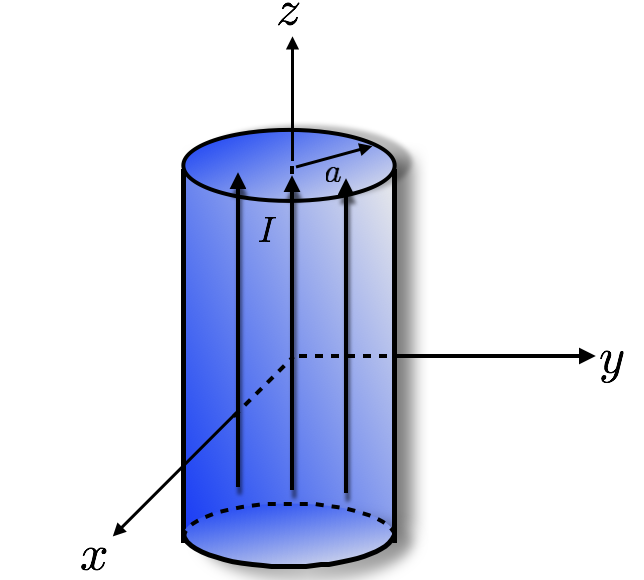
\includegraphics[scale=0.45]{Pictures/cilindrocorrientei.png}
\caption{\textit{Cilindro conductor de radio a.}}
\end{figure}

\emph{Soluci\'on}.\\\\
Sabemos que el cilindro es un conductor, por lo tanto la densidad de corriente libre $\textbf{J}_{f}=\sigma\textbf{E}$, donde $\sigma$ es la conductividad del cilindro. Por lo tanto podemos ver que $\textbf{E}=\frac{\textbf{J}_{f}}{\sigma}$, entonces para nuestro problema:
\begin{equation}
\textbf{E}=\frac{J_{f}}{\sigma}\hat{\textbf{z}}.  \label{Campo E}
\end{equation}
Por otro lado, se necesita calcular $\textbf{H}$, en la superficie del conductor, esto se puede hacer calculando el flujo magn\'etico $\textbf{B}$, a partir de la ley de Ampère en su forma integral, esto es:
\begin{eqnarray*}
\oint_{C}\textbf{B}\cdot d\textbf{l}=\mu_{0}I_{enc}.
\end{eqnarray*}
Si tomamos una secci\'on de integraci\'on normal a la densidad de corriente, esto es una curva $C$ que sea una circunferencia de radio $\rho$ $(\rho<a),$ con centro en el eje $z$.\\
El problema magn\'etico es similar en varias aspectos al el\'ectrico. Por simetr\'ia el campo magn\'etico sólo depende de la coordenada $\rho$. Por la similitud con la geometría de un hilo infinito, podemos suponer que es acimutal, es decir, $\textbf{B}=B_{\varphi}(\rho)\hat{\mathbf{\varphi}}$,
\begin{eqnarray*}
\oint_{C}\textbf{B}\cdot d\textbf{l}=\int_{C}B_{\varphi}(\rho)\rho d\varphi,
\end{eqnarray*}
\begin{eqnarray*}
\oint_{C}\textbf{B}\cdot d\textbf{l}=B_{\varphi}(\rho)\rho\int_{0}^{2\pi} d\varphi.
\end{eqnarray*}
Entonces:
\begin{eqnarray*}
B_{\varphi}(\rho)2\pi\rho=\mu_{0}I_{enc}.
\end{eqnarray*}
Por lo tanto:
\begin{eqnarray*}
B_{\varphi}(\rho)=\frac{\mu_{0}I_{enc}}{2\pi\rho}.
\end{eqnarray*}
Recordando que el campo magn\'etico es $\textbf{H}=\frac{\textbf{B}}{\mu_{0}}$, por otro lado, para el caso cuando $\rho\geq a$, entonces $I_{enc}=I$, adem\'as, de la definici\'on $J_{f}=\frac{I}{\pi a^{2}}$, entonces $\textbf{H}$ se puede escribir como:
\begin{equation}
\textbf{H}=\frac{aJ_{f}}{2}\hat{\varphi}. \label{Campo H}
\end{equation}
Sustituyendo las ecuaciones (\ref{Campo E}) y (\ref{Campo H}) en la expresi\'on para el vector de Poynting:
\begin{eqnarray*}
\textbf{S}=\left(\frac{J_{f}}{\sigma}\hat{z}\right)\times\left( \frac{aJ_{f}}{2}\hat{\varphi} \right).
\end{eqnarray*}
Por lo tanto, el vector de Poynting es:
\begin{equation}
\textbf{S}=-\frac{a J_{f}^{2}}{2\sigma}\hat{\rho}. \label{S}
\end{equation}
Si calculamos el flujo de la densidad de corriente de energ\'ia que fluye hacia dentro del cilindro, esto es:
\begin{eqnarray*}
-\oint_{S}\textbf{S}\cdot d\textbf{s}=-Sa\int  dz d\theta=-2aL\pi S=-\frac{a J_{f}^{2}}{2\sigma}(2aL\pi).
\end{eqnarray*}
 Ahora si calculamos la potencia W, la potencia que se disipa por calor:
\begin{eqnarray*}
\int_{V} \textbf{J}\cdot\textbf{E} \hspace{1mm} d\text{v}=\int_{V} \sigma E^{2} d\text{v}=\frac{a J_{f}^{2}}{2\sigma}(2aL\pi).
\end{eqnarray*}
 Por lo tanto la rapidez con la que fluye la energ\'ia hacia dentro del conductor es igual a la que se disipa por medio de calor. Esto es justo lo que se esperara para un sistema estacionario.

\end{example}

\begin{example}
Un cable coaxial ideal est\'a formado por un cilindro interior de radio $R_{1}$, perfectamente conductor y una superficie cil\'indrica exterior de radio $R_{2}$ tambi\'en perfectamente conductora. Los cilindros se extienden indefinidamente a lo largo de su eje.
El cilindro interior se encuentra a un potencial $\phi_{0}$, mientras que la superficie exterior se encuentra a tierra. Simult\'aneamente, por la superficie del n\'ucleo fluye una corriente $I$ en la direcci\'on del eje distribuida uniformemente. Esta corriente retorna por la superficie exterior, con lo que hay distribuida uniformemente una corriente $-I$.\\

\begin{itemize}
\item Halle los campos el\'ectrico y magn\'etico en todos los puntos del espacio.
\end{itemize}
\begin{itemize}
\item Calcule las densidades de energ\'ia el\'ectrica y magn\'etica por unidad de volumen, as\'i como la energ\'ia total almacenada en una porci\'on de longitud $L$ del cable coaxial.
\end{itemize}
\begin{itemize}
\item Determine el vector de Poynting en el espacio entre los cilindros. ¿En qu\'e direcci\'on fluye la energ\'ia?
\end{itemize}
\begin{itemize}
\item Halle el flujo de energ\'ia a trav\'es de una secci\'on del cable coaxial.
\end{itemize}

\begin{figure}[hbtp]
\centering
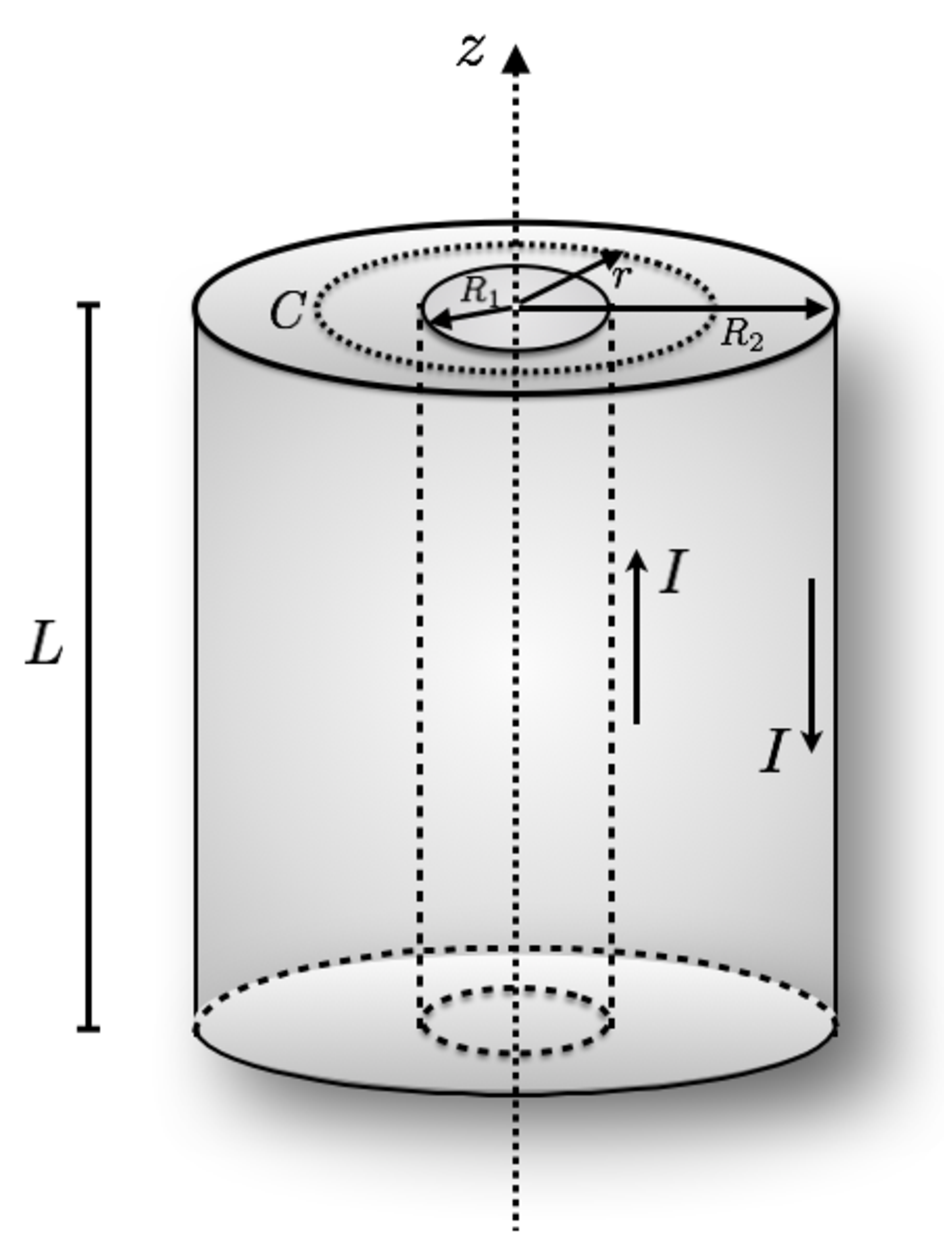
\includegraphics[scale=0.45]{Pictures/cascaras-cilindricas-coaxiales-con-corriente.pdf}
\caption{\textit{Cascaras cil\'indricas coaxiales con corriente.}}
\end{figure}

\emph{Soluci\'on}\\\\
%****************** Ejemplo *********************+++
Para el primer punto; considerando $L$ muy grande y considerando simetr\'ia con respecto a $\varphi$, tenemos que encontrar los campos el\'ectricos y magn\'eticos en todo el espacio. Primero calculamos el campo el\'ectrico $\textbf{E}$:\\
Dada la simetr\'ia cil\'indrica del problema, escogemos el eje $z$ coincidente con el eje central del cable. Resolveremos entonces la ecuaci\'on del potencial electrost\'atico en cada regi\'on definida por los conductores.\\Por la simetr\'ia del sistema el potencial en cada regi\'on s\'olo puede depender de la coordenada radial cil\'indrica $\rho$.\\
Para la regi\'on $\rho < R_{1}$, se tiene que el cable est\'a sometido a un potencial $\phi(\rho)=\varphi{0}$ es decir esa regi\'on es equipotencial en todos sus puntos. Por lo tanto, como podemos expresar el campo $\textbf{E}$ en t\'erminos del potencial como:
\begin{eqnarray*}
\textbf{E}=-\nabla\phi.
\end{eqnarray*}
Entonces el campo el\'ectrico es esta regi\'on es:
\begin{equation}
\textbf{E}=\textbf{0} \hspace{2cm}  \rho < R_{1}.  \label{E}
\end{equation}

Para la regi\'on $R_{1}< \rho < R_{2}$, se tiene la ecuaci\'on de Laplace pues no hay cargas libres,
\begin{eqnarray*}
\nabla^{2}\phi=0.
\end{eqnarray*}
Por lo tanto al usar coordenadas cil\'indricas:
\begin{eqnarray*}
\frac{1}{\rho}\frac{\partial}{\partial \rho}\left(\rho \frac{\partial\phi}{\partial \rho} \right)=0,
\end{eqnarray*}
entonces:
\begin{eqnarray*}
\frac{\partial}{\partial \rho}\left(\rho \frac{\partial\phi}{\partial \rho} \right)=0
\end{eqnarray*}
Por lo tanto el t\'ermino entre par\'entesis es una constante para $\rho$, la ecuaci\'on se puede escribir como:
\begin{eqnarray*}
\rho \frac{\partial \phi}{\partial \rho}=A \hspace{2cm} \text{con A-cte.}
\end{eqnarray*}
Por lo tanto al resolver la ecuaci\'on diferencial, obtenemos:
\begin{eqnarray}
\phi(\rho)=A\hspace{1mm}\ln(\rho)+B \hspace{2cm} \label{potenciale} \text{con B-cte.}
\end{eqnarray}
Esta ecuaci\'on esta sometida a condiciones de frontera; $\phi(R_{1})=V_{0}$ y $\phi(R_{2})=0$, por lo tanto al aplicar estas condiciones a la soluci\'on de $\phi$, obtenemos que las constates A y B son:
\begin{eqnarray*}
A=-\frac{V_{0}}{\ln\left( \frac{R_{2}}{R_{1}} \right)} \hspace{2cm} B=V_{0}-A\hspace{1mm}\ln(R_{1}).
\end{eqnarray*}
Entonces el potencial el\'ectrico es de la forma:
\begin{eqnarray*}
\phi(\rho)=-\frac{V_{0}}{\ln\left( \frac{R_{2}}{R_{1}} \right)}\ln\left( \frac{\rho}{R_{1}} \right)+V_{0}.
\end{eqnarray*}
Por lo tanto el campo el\'ectrico est\'a dado por:
\begin{eqnarray*}
\textbf{E}=-\nabla\phi=-\frac{\partial}{\partial \rho}\left(-\frac{V_{0}}{\ln\left( \frac{R_{2}}{R_{1}} \right)}\ln\left( \frac{\rho}{R_{1}} \right)+V_{0}\right)\hat{\rho},
\end{eqnarray*}
\begin{equation}
\textbf{E}=\frac{V_{0}}{\rho \hspace{1mm}\ln\left( \frac{R_{2}}{R_{1}} \right)}\hat{\rho} \hspace{2cm}R_{1}< \rho < R_{2}.  \label{E2}
\end{equation}
En la regi\'on $\rho > R_{2}$, aqu\'i tampoco hay carga, por lo que el potencial tiene la misma forma que que (\ref{potenciale}). Las condiciones de frontera son homog\'eneas, pues $\phi(R_{2})=0$ y $\phi(\rho\to1)=0.$
Entonces el potencial es nulo y por tanto el campo el\'ectrico tambi\'en.\\
Por lo tanto el campo el\'ectrico en todo el espacio es:
\begin{equation}
\mathbf{E}=\begin{cases} \textbf{0}, & \rho<R_{1},\\ & \\ \displaystyle\frac{V_0}{\ln(R_{2}/R_{1})}\frac{1}{\rho}\hat{\rho}, &R_{1}<\rho<R_2, \\ & \\ \textbf{0}, & \rho>R_{2}.\end{cases}  \label{E en espacio}
\end{equation}
El problema para el campo magn\'etico es similar en varias aspectos al el\'ectrico. Por simetr\'ia el campo magn\'etico s\'olo depende de la coordenada $\rho$. Por la similitud con la geometr\'ia de un hilo infinito, podemos suponer que es acimutal. Podemos utilizar la ley de Ampère en su forma integral para resolver el problema.
\begin{eqnarray*}
\oint_C \textbf{B}  \cdot d \textbf{l}=\mu_{0} I_{enc},
\end{eqnarray*}
siendo $I_{enc}$ la corriente que atraviesa una superficie que encierra el contorno de circulaci\'on de $\textbf{B}$.\\
Consideramos circunferencias contenidas en planos perpendiculares al eje $z$, conc\'entricas con \'el de radio $\rho$, entonces:
\begin{equation}
 \oint_C\mathbf{B}\cdot \mathrm{d}\textbf{l} = 2\pi\rho B(\rho) \quad\Rightarrow\quad B(\rho) = \frac{\mu_0 I_{enc}}{2\pi\rho}.
\end{equation}
Por lo tanto, para el caso cuando $\rho<R_{1}$, se tiene que no hay corriente que atraviese la superficie, pues el problema indica que la corriente se distribuye uniformemente sobre la superficie el cilindro interior. Entonces $I_{enc}=0$, por lo tanto el campo magn\'etico en esta regi\'on es:
\begin{equation}
 \textbf{B}=\textbf{0}.  \label{B}
\end{equation}
Para el caso cuando $R_{1}<\rho<R_{2}$, la corriente que pasa por la superficie es $I_{enc}=I$, entonces el campo magn\'etico esta dado por:
\begin{equation}
\textbf{B}=\frac{\mu_0 I}{2\pi\rho}\hat{\varphi}.
\end{equation}
Por \'ultimo para la regi\'on $\rho>R_{2}$, se tiene las dos corrientes que pasan por los dos cilindros, pero como una es igual que la otro pero en sentido contrario, la corriente neta es cero, por lo tanto $I_{enc}=0$. Entonces el campo magn\'etico es:
\begin{equation}
 \textbf{B}=\textbf{0}.
\end{equation}
Resumiendo, el campo magn\'etico en todo el espacio es:
\begin{equation}
\mathbf{B}=\begin{cases} \textbf{0,} & \rho<R_{1},\\ & \\ \displaystyle \frac{\mu_0 I}{2\pi\rho}\hat{\varphi}, & R_{1}<\rho<R_{2}, \\ & \\ \textbf{0}, & \rho>R_{2}.\end{cases}
\end{equation}
Para el segundo punto, esto es, calcular las densidades de energ\'ia el\'ectrica y magn\'etica en el cable coaxial. Una observaci\'on que se puede hacer, es que las densidades se anulan en todas las regiones a excepci\'on de $R_{1}<\rho<R_{2}$, ya que es el \'unico lugar en donde los campos no son nulos.\\
Para calcular las densidades de energ\'ia, ocupamos las expresiones:
\begin{eqnarray*}
u_{e}=\frac{\epsilon_{0}}{2}E^{2},
\end{eqnarray*}
\begin{eqnarray*}
u_{m}=\frac{\mu_{0}}{2}H^{2}.
\end{eqnarray*}
Por lo tanto la densidad de energ\'ia el\'ectrica es:
\begin{equation}
\begin{split}
u_{e}&=\frac{\epsilon_{0}}{2}E^{2},\\
&=\frac{\epsilon_{0}}{2}\left( \frac{V_{0}}{\rho \hspace{1mm}\ln\left( \frac{R_{2}}{R_{1}} \right)} \right)^{2},\\
&=\frac{\epsilon_{0}}{2} \frac{V_{0}^{2}}{\rho^{2} \hspace{1mm}\ln^{2}\left( \frac{R_{2}}{R_{1}} \right)}.
\end{split}
\end{equation}
Por la tanto, para obtener la energ\'ia el\'ectrica almacenada $U_{e}$ en una secci\'on de longitud $L$ del cilindro, se necesita integrar la densidad de energ\'ia $u_{e}$, en un volumen $V$, esto es:
\begin{eqnarray*}
U_{e}=\int_{0}^{L}\int_{0}^{2\pi}\int_{R_{1}}^{R_{2}}\frac{\epsilon_{0}}{2} \frac{V_{0}^{2}}{\rho^{2} \hspace{1mm}\ln^{2}\left( \frac{R_{2}}{R_{1}} \right)}\rho d\rho d\varphi dz.
\end{eqnarray*}
Al realizar la integral respecto al \'angulo $d\varphi$ y la coordenada $dz$, entonces
\begin{eqnarray*}
\int_{R_{1}}^{R_{2}}\frac{2\pi L\epsilon_{0}}{2} \frac{V_{0}^{2}}{\rho \hspace{1mm}\ln^{2}\left( \frac{R_{2}}{R_{1}} \right)} d\rho.
\end{eqnarray*}
Simplificando un poco la expresi\'on:
\begin{eqnarray*}
\frac{V_{0}^{2}\pi L\epsilon_{0}}{\ln^{2}\left( \frac{R_{2}}{R_{1}} \right)}\int_{R_{1}}^{R_{2}} \frac{d\rho}{\rho}.
\end{eqnarray*}
Entonces, al realizar la integral directa:
\begin{eqnarray*}
\frac{V_{0}^{2}\pi L\epsilon_{0}}{\ln^{2}\left( \frac{R_{2}}{R_{1}} \right)} \ln\left(\frac{R_{2}}{R_{1}}\right).
\end{eqnarray*}
Por lo tanto la energ\'ia el\'ectrica almacenada es:
\begin{equation}
U_{e}=\frac{V_{0}^{2}\pi L\epsilon_{0}}{\ln\left( \frac{R_{2}}{R_{1}} \right)}.
\end{equation}
Ahora para calcular la energ\'ia magn\'etica almacenada, utilizamos la expresi\'on:
\begin{eqnarray*}
U_{m}=\int_{V} u_{m}\hspace{1mm} d\text{v}=\int_{V}\frac{\mu_{0}}{2}H^{2}\hspace{1mm}d\text{v}.
\end{eqnarray*}
Al susutitur la expresi\'on para el campo magn\'etico encontrado antes y recordando que $\textbf{H}=\frac{\textbf{B}}{\mu_{0}}$, entonces:
\begin{eqnarray*}
U_{m}=\int_{V}\frac{\mu_{0}}{2}\left( \frac{I}{2\pi\rho} \right)^{2}\hspace{1mm}d\text{v}.
\end{eqnarray*}
Al calcular la integral en el volumen $V$ en coordenadas cil\'indricas:
\begin{eqnarray*}
\int_{0}^{L}\int_{0}^{2\pi}\int_{R_{1}}^{R_{2}}\frac{\mu_{0}}{2} \frac{I^{2}}{4\pi^{2}\rho^{2}} \hspace{1mm}\rho d\rho d\varphi dz.
\end{eqnarray*}
De nuevo primero calculamos las integrales respecto a $d\varphi$ y $dz$
\begin{eqnarray*}
\frac{2\pi L \mu_{0}}{2} \frac{I^{2}}{4\pi^{2}}\int_{R_{1}}^{R_{2}} \frac{d\rho}{\rho}.
\end{eqnarray*}
simplificando un poco y calculando la integral respecto a $\rho$, obtenemos:
\begin{equation}
U_{m}=\frac{I^{2} L \mu_{0}}{4\pi} \ln\left( \frac{R_{2}}{R_{1}} \right).
\end{equation}
Por lo tanto la energ\'ia electromagn\'etica total almacenada en una secci\'on de longitud $L$ del cable coaxial es:
\begin{equation}
U=U_{e}+U_{m}=\frac{V_{0}^{2}\pi L\epsilon_{0}}{ln\left( \frac{R_{2}}{R_{1}} \right)}+\frac{I^{2} L \mu_{0}}{4\pi} ln\left( \frac{R_{2}}{R_{1}} \right).
\end{equation}
Por \'ultimo, para calcular el vector de Poynting, usamos la ec. (\ref{Vector S}), adem\'as como solo para la regi\'on entre los dos cilindros los campos no son nulos, entonces el vector de Poynting est\'a en esa regi\'on.
\begin{eqnarray*}
\textbf{S}=\textbf{E}\times\textbf{H}.
\end{eqnarray*}
Sustituyendo las expresiones para los campos $\textbf{E}$ y $\textbf{H}$ encontradas antes, obtenemos:
\begin{eqnarray*}
\textbf{S}=\left( \frac{V_0}{\ln(R_{2}/R_{1})}\frac{1}{\rho}\hat{\rho} \right)\times\left( \frac{I}{2\pi\rho}\hat{\varphi} \right).
\end{eqnarray*}
Por lo tanto el vector $\textbf{S}$, est\'a dado por:
\begin{equation}
\textbf{S}=\frac{IV_0}{2\pi\rho^{2}\ln(R_{2}/R_{1})}\hat{z}.
\end{equation}
Si $V_{0}$ es positivo, la energ\'ia se transmite entonces en el sentido positivo del eje z, es decir, en la direcci\'on en que fluye la corriente en el n\'ucleo del cable.\\
Para calcular la potencia transmitida a trav\'es de una secci\'on del cable hay que calcular el flujo del vector de Poynting en esa secci\'on, esto es:
\begin{eqnarray*}
P=\oint_{s} \textbf{S}\cdot \hspace{1mm}d\textbf{a}=\oint_{s}\frac{IV_0}{2\pi\rho^{2}\ln(R_{2}/R_{1})}\hat{z} \cdot \hat{z}\hspace{1mm}d\textbf{a}.
\end{eqnarray*}
Al calcular la integral de superficie en coordenadas cil\'indricas:
\begin{eqnarray*}
P=\frac{IV_0}{2\pi\ln(R_{2}/R_{1})}\int_{R_{1}}^{R_{2}}\int_{0}^{2\pi}\hspace{1mm}\frac{1}{\rho} d\rho d\varphi.
\end{eqnarray*}
Al realizar la integral respecto al \'angulo polar, obtenemos:
\begin{eqnarray*}
P=\frac{IV_0}{\ln(R_{2}/R_{1})}\int_{R_{1}}^{R_{2}}\hspace{1mm}\frac{1}{\rho} d\rho.
\end{eqnarray*}

Por lo tanto la potencia transmitida por de una secci\'on del cable en el eje $z$ es:
\begin{equation}
P=IV_{0}.
\end{equation}
\end{example}

%*********************SECCION********************
\section{Tensor de esfuerzo de Maxwell en el campo electromagn\'etico}

En la mec\'anica de Newton, sabemos que la variaci\'on del momento lineal nos cuantifica la interacci\'on entre dos part\'iculas a trav\'es de una fuerza, por lo tanto, es razonable pensar que ocurre lo mismo en los fen\'omenos electromagnetismos.\\ Para esto se parte de la idea de estudiar la fuerza electromagn\'etica; dado que estamos trabajando con un medio continuo (distribuciones continuas de carga) y la fuerza se distribuye de forma continua en el volumen de la distribuci\'on, es mas \'util comenzar con el concepto de densidad de fuerza.\\\\
Dado que la fuerza electromagn\'etica para una carga puntual $q$ est\'a dada por la fuerza de Lorentz:
\begin{eqnarray*}
\textbf{F}=q(\textbf{E}+\textbf{v}\times\textbf{B}).
\end{eqnarray*}

Como esta fuerza va a cambiar dependiendo en que parte del volumen considerado se est\'e aplicando, entonces podemos definir una densidad de fuerza $\textbf{f}$ como $\textbf{f}=\frac{d \textbf{f}}{dV}$, entonces podemos escribir a $\textbf{f}$ como:
\begin{eqnarray*}
\textbf{f}=\frac{dq}{dV}(\textbf{E}+\textbf{v}\times\textbf{B}).
\end{eqnarray*}
Y como la variaci\'on de la carga en un volumen dado es justamente la densidad de carga, entonces:
\begin{equation}
\textbf{f}=\rho\textbf{E}+\textbf{J}\times\textbf{B}.
\end{equation}
Ahora es conveniente escribir la densidad de fuerza en funci\'on de los campos el\'ectricos y magn\'eticos. Para esto usamos las ecuaciones de Maxwell para despejar las fuentes de carga y densidad de corriente, de modo que:
\begin{eqnarray*}
\rho=\epsilon_{0}\nabla\cdot\textbf{E},
\end{eqnarray*}
\begin{eqnarray*}
\textbf{J}=\frac{1}{\mu_{0}}\nabla\times\textbf{B}-\epsilon_{0}\frac{\partial \textbf{E}}{\partial t}.
\end{eqnarray*}
Entonces la densidad de fuerza se puede reescribir como:
\begin{equation}
\textbf{f}=(\epsilon_{0}\nabla\cdot\textbf{E})\textbf{E}+\left( \frac{1}{\mu_{0}}\nabla\times\textbf{B}-\epsilon_{0}\frac{\partial \textbf{E}}{\partial t} \right)\times\textbf{B}.
\end{equation}
Desarrollando el producto vectorial y agrupando t\'erminos
\begin{eqnarray*}
\textbf{f}=(\epsilon_{0}\nabla\cdot\textbf{E})\textbf{E}+ \frac{1}{\mu_{0}}(\nabla\times\textbf{B})\times\textbf{B}-\epsilon_{0}\frac{\partial \textbf{E}}{\partial t} \times\textbf{B},
\end{eqnarray*}
\begin{equation}
\textbf{f}=\epsilon_{0}\left((\nabla\cdot\textbf{E})\textbf{E}-\frac{\partial \textbf{E}}{\partial t} \times\textbf{B}\right) +\frac{1}{\mu_{0}}(\nabla\times\textbf{B})\times\textbf{B}. \label{Desidad de Fuerza}
\end{equation}


%--------------Obs---------------
\begin{obs}
Por otro lado podemos ver que para dos vectores cualesquiera $\textbf{E}$ y $\textbf{B}$ se tiene que:
\begin{eqnarray*}
\frac{\partial}{\partial t}(\textbf{E}\times\textbf{B})=\left( \frac{\partial\textbf{E}}{\partial t}\times\textbf{B}\right)+\left(\textbf{E}\times\frac{\partial\textbf{B}}{\partial t}\right).
\end{eqnarray*}

Entonces:
\begin{eqnarray*}
\frac{\partial\textbf{E}}{\partial t}\times\textbf{B}=\frac{\partial}{\partial t}(\textbf{E}\times\textbf{B})-\textbf{E}\times\frac{\partial\textbf{B}}{\partial t}.
\end{eqnarray*}
\end{obs}


Ahora para el segundo t\'ermino del lado derecho de la expresi\'on anterior, sustituimos la ley  de Faraday $\nabla\times\textbf{E}=-\frac{\partial  \textbf{B}}{\partial t}$, obtenemos:
\begin{equation}
\frac{\partial\textbf{E}}{\partial t}\times\textbf{B}=\frac{\partial}{\partial t}(\textbf{E}\times\textbf{B})+\textbf{E}\times(\nabla\times\textbf{E}).
\end{equation}
Si sustituimos esta \'ultima expresi\'on en la ec. (\ref{Desidad de Fuerza})
\begin{eqnarray*}
\textbf{f}=\epsilon_{0}\left((\nabla\cdot\textbf{E})\textbf{E}-\left[\frac{\partial}{\partial t}(\textbf{E}\times\textbf{B})+\textbf{E}\times(\nabla\times\textbf{E}) \right]\right) +\frac{1}{\mu_{0}}(\nabla\times\textbf{B})\times\textbf{B},
\end{eqnarray*}
ordenando un poco los t\'erminos
\begin{equation}
\textbf{f}=\epsilon_{0}\left[(\nabla\cdot\textbf{E})\textbf{E}-\textbf{E}\times(\nabla\times\textbf{E})\right] +\frac{1}{\mu_{0}}(\nabla\times\textbf{B})\times\textbf{B}-\epsilon_{0}\frac{\partial}{\partial t}(\textbf{E}\times\textbf{B}).
\end{equation}
Para que la expresi\'on anterior tenga un poco m\'as de simetr\'ia, le sumamos una cantidad tal que, mantenga inalterable la igualdad. Esto se logra introduciendo la ley de Gauss para el campo magn\'etico, es decir, sumando $(\nabla\cdot\textbf{B})\textbf{B}$; ya que la divergencia del campo magn\'etico es siempre es cero; por lo tanto podemos escribir la densidad de fuerza electromagn\'etica como:
\begin{equation}
\textbf{f}=\epsilon_{0}\left[(\nabla\cdot\textbf{E})\textbf{E}-\textbf{E}\times(\nabla\times\textbf{E})\right] +\frac{1}{\mu_{0}}\left[(\nabla\cdot\textbf{B})\textbf{B}-\textbf{B}\times(\nabla\times\textbf{B})\right]-\epsilon_{0}\frac{\partial}{\partial t}(\textbf{E}\times\textbf{B}). \label{Dens fuerza}
\end{equation}
Ahora usamos la identidad vectorial:
\begin{eqnarray*}
\nabla(E^{2})=2(\textbf{E}\cdot\nabla)\textbf{E}+2\textbf{E}(\nabla\times\textbf{E}).
\end{eqnarray*}
De modo que:
\begin{equation}
\textbf{E}(\nabla\times\textbf{E})=\frac{1}{2}\nabla(E^{2})-(\textbf{E}\cdot\nabla)\textbf{E}.
\end{equation}
Al sustituir esta expresi\'on en la ec. (\ref{Dens fuerza}), obtenemos:
\begin{equation}
\textbf{f}=\epsilon_{0}\left[(\nabla\cdot\textbf{E})\textbf{E}-\frac{1}{2}\nabla(E^{2})+(\textbf{E}\cdot\nabla)\textbf{E}\right] +\frac{1}{\mu_{0}}\left[(\nabla\cdot\textbf{B})\textbf{B}-\frac{1}{2}\nabla(B^{2})+(\textbf{B}\cdot\nabla)\textbf{B}\right]-\epsilon_{0}\frac{\partial}{\partial t}(\textbf{E}\times\textbf{B}),  \label{Dens Fuerza 2}
\end{equation}
est\'a expresi\'on es bastante complicada de manejar por lo que se recurre a definir una nueva cantidad llamada, \textit{tensor de esfuerzo de Maxwell} \cite{Griffiths1999}, definido como:
\begin{equation}
T_{ij}=\epsilon_{0}\left(E_{i}E_{j}-\frac{1}{2}\delta_{ij}E^{2}\right)+\frac{1}{\mu_{0}}\left(B_{i}B_{j}-\frac{1}{2}\delta_{ij}B^{2}\right),  \label{Tensor de Esfuerzo}
\end{equation}
donde los \'indices $i$ y $j$ hacen referencia a las coordenadas $x$, $y$, $z$  as\'i el tensor de esfuerzo tiene en total $9$ componentes.\\\\
Por ejemplo, para el vector tridimensional $\textbf{A}$,
\begin{eqnarray*}
A_x=A_1, \hspace{2mm} A_y=A_2, \hspace{2mm} A_z=A_3
\end{eqnarray*}

Podemos representar esta nueva cantidad como si fuera una especie de matriz, entonces se define la componente $i$ del producto de $\textbf{T}$ con cualquier vector $\textbf{a}$ como:
\begin{equation}
(\textbf{a}\cdot\textbf{T})_{i}=\sum_{j=x,y,z} a_{j}T_{ji}.
\end{equation}
De manera an\'aloga podemos escribir la componente $j$ de la divergencia de $\textbf{T}$, esto es:
\begin{eqnarray*}
(\nabla\cdot\textbf{T})_{j}=\sum_{i=x,y,z} \nabla_{i}T_{ij},
\end{eqnarray*}
\begin{eqnarray*}
(\nabla\cdot\textbf{T})_{j}=\sum_{i=x,y,z} \nabla_{i}\left[ \epsilon_{0}\left(E_{i}E_{j}-\frac{1}{2}\delta_{ij}E^{2}\right)+\frac{1}{\mu_{0}}\left(B_{i}B_{j}-\frac{1}{2}\delta_{ij}B^{2}\right) \right].
\end{eqnarray*}
Distribuyendo el operador $\nabla_{i}$ en todo el producto:
\begin{eqnarray*}
(\nabla\cdot\textbf{T})_{j}=\sum_{i=x,y,z} \left[ \epsilon_{0}\left( \nabla_{i}(E_{i}E_{j})-\frac{1}{2}\delta_{ij}\nabla_{i}(E^{2})\right)+\frac{1}{\mu_{0}}\left(\nabla_{i}(B_{i}B_{j})-\frac{1}{2}\delta_{ij}\nabla_{i}(B^{2})\right) \right],
\end{eqnarray*}
\begin{eqnarray*}
(\nabla\cdot\textbf{T})_{j}=\sum_{i=x,y,z} \left[ \epsilon_{0}\left( (\nabla_{i}E_{i})E_{j}+(E_{i}\nabla_{i})E_{j}-\frac{1}{2}\nabla_{j}(E^{2})\right)+\frac{1}{\mu_{0}}\left((\nabla_{i}B_{i})B_{j}+(B_{i}\nabla_{i})B_{j}-\frac{1}{2}\nabla_{j}(B^{2})\right) \right].
\end{eqnarray*}
Por otra parte podemos escribir el producto escalar de dos vectores como $\textbf{A}\cdot\textbf{B}=\sum_{i}A_{i}B_{i}$, entonces podemos reescribir la expresi\'on anterior como:
\begin{equation}
(\nabla\cdot\textbf{T})_{j}=\epsilon_{0}\sum_{i=x,y,z}\left[ (\nabla\cdot\textbf{E})E_{j}+(\textbf{E}\cdot\nabla)E_{j}-\frac{1}{2}\nabla_{j}(E^{2})\right)+\frac{1}{\mu_{0}}\left((\nabla\cdot\textbf{B})B_{j}+(\textbf{B}\cdot\nabla)B_{j}-\frac{1}{2}\nabla_{j}(B^{2})\right].
\end{equation}
Entonces sustituyendo esta igualdad, en la ec. (\ref{Dens Fuerza 2}), obtenemos una expresi\'on para la densidad de fuerza electromagn\'etica
\begin{equation}
\textbf{f}=\nabla\cdot\textbf{T}-\epsilon_{0}\frac{\partial}{\partial t}(\textbf{E}\times\textbf{B}).
\end{equation}
Adem\'as recordado que podemos escribir el campo $\textbf{B}$ como $\textbf{B}=\mu_{0}\textbf{H}$.
Entonces, la densidad de fuerza electromagn\'etica se escribe como:
\begin{equation}
\textbf{f}=\nabla\cdot\textbf{T}-\epsilon_{0}\mu_{0}\frac{\partial \textbf{S}}{\partial t}.
\end{equation}
Si se integra en un volumen $V$ encerrado por una superficie $S$, obtenemos la fuerza que es ejercida por los campos electromagn\'eticos en el volumen $V$,
\begin{eqnarray*}
\textbf{F}=\int_{V}\nabla\cdot\textbf{T}\hspace{1mm} d\text{v}-\epsilon_{0}\mu_{0}\frac{\partial}{\partial t}\int_{V} \textbf{S}\hspace{1mm} d\text{v}.
\end{eqnarray*}
Aplicando el teorema de la divergencia a la primera integral, obtenemos:
\begin{equation}
\textbf{F}=\oint_{S}\textbf{T}\cdot\hspace{0.5mm} d\textbf{s}-\epsilon_{0}\mu_{0}\frac{\partial}{\partial t}\int_{V} \textbf{S}\hspace{1mm} dv. \label{Fuerza}
\end{equation}
De esta forma podemos apreciar que f\'isicamente el tensor $\textbf{T}$ representa la fuerza por unidad de \'area en direcci\'on $i$ que es ejercida en un elemento de superficie en direcci\'on $j$.\\\\
Por otra parte, de acuerdo a la segunda ley de Newton, la fuerza que experimenta un cuerpo, es debida a la variaci\'on del momento lineal del cuerpo. Aplicando este principio a la fuerza electromagn\'etica, entonces obtenemos:
\begin{equation}
\frac{d \textbf{P}_{mec}}{dt}=\oint_{s}\textbf{T}\cdot\hspace{0.5mm} d\textbf{s}-\epsilon_{0}\mu_{0}\frac{\partial}{\partial t}\int_{V} \textbf{S}\hspace{1mm} d\text{v},
\end{equation}
donde $\textbf{P}_{mec}$ es el momento mec\'anico total de las cargas encerradas en el volumen $V$. Esta expresi\'on se similar a la del teorema de Poynting, por lo tanto, se puede obtener una interpretaci\'on similar.\\
Consideramos la segunda integral como el momento almacenado por los campos electromagn\'eticos.
Si llamamos $\textbf{g}=\epsilon_{0}\mu_{0}\textbf{S}$ a la densidad de momento lineal almacenada por los campos, entonces se puede escribir:
\begin{equation}
 \textbf{P}_{em}=\int_{V} \textbf{g}\hspace{1mm} d\text{v}.
 \end{equation}
Ahora la primera integral debe darnos el flujo del momento lineal por unidad de tiempo que fluye por la superficie del volumen. La expresi\'on (\ref{Fuerza}), nos representa una forma general de la conservaci\'on del momento lineal.
Por lo tanto, un incremento en el momento total es igual al flujo de momento por unidad de tiempo creado por los campos.
\begin{equation}
\frac{d}{dt}(\textbf{P}_{mec}+\textbf{P}_{em})=\oint_{s}\textbf{T}\cdot\hspace{0.5mm} d\textbf{s}.
\end{equation}
Cuando se calcula esa integral de flujo en todo el espacio, vemos que no hay contribuci\'on del flujo de momento, por lo tanto:
\begin{equation}
\textbf{P}_{mec}+\textbf{P}_{em}=\text{cte},
\end{equation}
es decir, cuando se toman todas las contribuciones del espacio y no solo una regi\'on entonces se da la conservaci\'on del momento lineal mec\'anico y electromagn\'etico.\\\\


%******************** Ejemplo******************************+
\begin{example}
Determinar la fuerza que ejercen los campos electromagn\'eticos sobre el hemisferio norte de una esfera solida con una densidad de carga volum\'etrica uniforme de radio $R$. \\\\
\begin{figure}[hbtp]
\centering
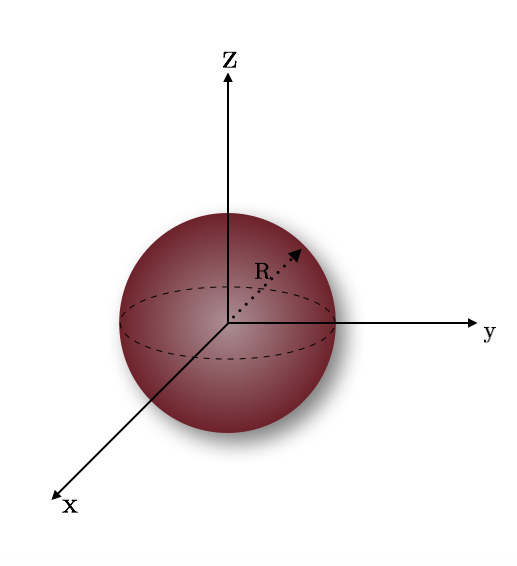
\includegraphics[scale=0.55]{Pictures/esferault.png}
\caption{\textit{Esfera de radio $R$.}}
\end{figure}

\emph{Soluci\'on}.
%************************* Solucion *************************
\\\\Para calcular la fuerza en el hemisferio norte de la esfera, tenemos que ocupar la ec. (\ref{Fuerza}), usando el tensor de esfuerzo de Maxwell. Entonces,
\begin{eqnarray*}
\textbf{F}=\oint_{s}\textbf{T}\cdot\hspace{0.5mm} d\textbf{s}-\epsilon_{0}\mu_{0}\frac{\partial}{\partial t}\int_{V} \textbf{S}\hspace{1mm} d\text{v}.
\end{eqnarray*}
Adem\'as necesitamos obtener el campo el\'ectrico, en la superficie y dentro de la parte norte de la esfera. Para la superficie:\\
Recordemos que podemos obtener el campo el\'ectrico en la superficie como si toda la carga estuviera concentrada en el origen de coordenadas, es decir, el campo el\'ectrico de una carga puntual $Q$ a una distancia $R$, entonces:
\begin{equation}
\textbf{E}=\frac{1}{4\pi\epsilon_{0}}\frac{Q}{R^{2}}\hat{\textbf{r}}.
\end{equation}
Para calcular el campo el\'ectrico dentro de la esfera, partimos por la ley de Gauss, consideramos una superficie gaussiana com\'un radio $r<R$, adem\'as podemos considerar que $\textbf{E}$ es radial, entonces $\textbf{E}=E_{r}\hat{\textbf{r}}$.
\begin{eqnarray*}
\oint_{s} \textbf{E}\cdot\,d\textbf{s}=\frac{1}{\epsilon_{0}}\int_{V}\rho d\text{v}.
\end{eqnarray*}
Como la densidad de carga volum\'etrica es constante, entonces $Q_{enc}=\frac{4}{3}\rho \pi r^{3}$, por lo tanto
\begin{eqnarray*}
E_{r}4\pi r^{2}=\frac{4\rho \pi r^{3}}{3\epsilon_{0}}.
\end{eqnarray*}
 Recordando que la densidad volum\'etrica es $\rho=\frac{3Q}{4 \pi  Ŗ^{3}}$, entonces el campo el\'ectrico dentro de la esfera es:
\begin{equation}
 \textbf{E}=\frac{1}{4 \pi \epsilon_{0}}\frac{Qr}{R^{3}}\hat{\textbf{r}}.
\end{equation}
Como no hay cargas en movimiento, el campo $\textbf{B}$ es cero, por lo tanto el vector de Poynting es nulo, entonces la fuerza la podemos expresar como:
\begin{equation}
\textbf{F}=\oint_{s}\textbf{T}\cdot\hspace{0.5mm} d\textbf{s}. \label{Fuerza-tensor}
\end{equation}
Primero hay que obtener las componentes del tensor de esfuerzo de Maxwell, pero por simetr\'ia del sistema, solo hay contribuciones en el eje $z$, por lo tanto, los las \'unicas componentes del tensor que no son nulas son: $T_{zx}$, $T_{zy}$ y $T_{zz}$.\\ Recordando que el tensor de esfuerzo, para este problema tiene la forma:
\begin{equation}
 \textbf{T}_{ij}=\epsilon_{0}\left( E_{i}E_{j}-\frac{1}{2}\delta_{ij}E^{2} \right). \label{prueba}
\end{equation}
 Entonces para el campo el\'ectrico en la superficie:
\begin{eqnarray*}
\textbf{E}=\frac{1}{4\pi\epsilon_{0}}\frac{Q}{R^{2}} (\sen \theta \cos \varphi \hat{\textbf{i}}+\sen \theta \sen \varphi \hat{\textbf{j}}+\cos \theta \hat{\textbf{k}}).
\end{eqnarray*}
 Entonces las componentes del tensor de esfuerzo son:
\begin{equation}
T_{zx}=\epsilon_{0}\left(\frac{Q}{4 \pi \epsilon_{0}R^{2}} \right)^{2}\sen \theta \cos \varphi cos \theta.
\end{equation}
\begin{equation}
T_{zy}=\epsilon_{0}\left(\frac{Q}{4 \pi \epsilon_{0}R^{2}} \right)^{2}\sen \theta \sin \varphi \cos \theta.
\end{equation}
\begin{eqnarray*}
T_{zz}=\frac{\epsilon_{0}}{2}\left(\frac{Q}{4 \pi \epsilon_{0}R^{2}} \right)^{2}\left(\cos^{2} \theta- \sen^{2} \theta \cos^{2} \varphi- \sen^{2} \theta \sen^{2} \varphi\right).
\end{eqnarray*}
 \begin{equation}
 T_{zz}=\frac{\epsilon_{0}}{2}\left(\frac{Q}{4 \pi \epsilon_{0}R^{2}} \right)^{2}\left(\cos^{2} \theta- \sen^{2}\theta\right).
 \end{equation}
Por otro lado, al tener simetr\'ia sobre el eje $z$, entonces el producto escalar $\textbf{T}\cdot d\textbf{s}=(T\hspace{1mm}ds)_{z}$. Por lo tanto:
\begin{eqnarray*}
\textbf{T}\hspace{1mm}\cdot d\textbf{s}=\epsilon_{0}\left(\frac{Q}{4 \pi \epsilon_{0}R^{2}} \right)^{2}R^{2}\sen \theta \cos \theta d\theta d\varphi\left(\sen^{2} \theta \cos^{2} \varphi+\sen^{2} \theta \sen^{2} \varphi+\frac{1}{2}(\cos^{2} \theta - \sen^{2} \theta)  \right).
\end{eqnarray*}
Factorizando un $\sen^{2} \theta$,
\begin{eqnarray*}
\textbf{T}\hspace{1mm}\cdot d\textbf{s}=\epsilon_{0}\left(\frac{Q}{4 \pi \epsilon_{0}R^{2}} \right)^{2}R^{2}\sen \theta \cos \theta d\theta d\varphi\left(\sen^{2} \theta (\cos^{2} \varphi+ \sen^{2} \varphi)+\frac{1}{2}(1-\sen^{2} \theta)- \frac{1}{2}\sen^{2} \theta  \right),
\end{eqnarray*}
\begin{eqnarray*}
\textbf{T}\hspace{1mm}\cdot d\textbf{s}=\epsilon_{0}\left(\frac{Q}{4 \pi \epsilon_{0}R^{2}} \right)^{2}R^{2}\sen \theta \cos \theta d\theta d\varphi\left(\sen^{2} \theta +\frac{1}{2}-\frac{1}{2}\sen^{2} \theta - \frac{1}{2}\sen^{2} \theta  \right),
\end{eqnarray*}
\begin{equation}
\textbf{T}\hspace{1mm}\cdot d\textbf{s}=\frac{\epsilon_{0}}{2}\left(\frac{Q}{4 \pi \epsilon_{0}R^{2}} \right)^{2}R^{2}\sen \theta \cos \theta d\theta d\varphi.
\end{equation}
al sustituir esta expresi\'on en la ec, (\ref{Fuerza-tensor}) obtenemos:
\begin{eqnarray*}
\textbf{F}=\int_{s} \frac{\hat{\textbf{z}}\epsilon_{0}}{2}\left(\frac{Q}{4 \pi \epsilon_{0}R^{2}} \right)^{2}R^{2}\sen \theta \cos \theta d\theta d\varphi.
\end{eqnarray*}
Al integrar en el hemisferio norte de la esfera, obtenemos:
\begin{eqnarray*}
\textbf{F}=\frac{\hat{\textbf{z}}\epsilon_{0}}{2}\left(\frac{Q}{4 \pi \epsilon_{0}R^{2}} \right)^{2}R^{2}\int_{0}^{\frac{\pi}{2}}\int_{0}^{2\pi} \sen \theta \cos \theta d\theta d\varphi,
\end{eqnarray*}
\begin{eqnarray*}
\textbf{F}=\frac{2\pi \hat{\textbf{z}}\epsilon_{0}}{2}\left(\frac{Q}{4 \pi \epsilon_{0}R^{2}} \right)^{2}R^{2}\int_{0}^{\frac{\pi}{2}} \sen \theta \cos \theta d\theta.
\end{eqnarray*}
Esta integral es inmediata, por lo que obtenemos es,
\begin{eqnarray*}
\textbf{F}=\frac{\pi \hat{\textbf{z}}\epsilon_{0}}{2}\left(\frac{Q}{4 \pi \epsilon_{0}R^{2}} \right)^{2}R^{2}.
\end{eqnarray*}
Simplificando t\'erminos,
\begin{equation}
\textbf{F}=\frac{1}{4 \pi \epsilon_{0}} \frac{Q^{2}}{8R^{2}} \hat{\textbf{z}}.
\end{equation}
Ahora para calcular la fuerza ejercida en el plano $xy$ dentro de la esfera necesitamos calcular primero el campo el\'ectrico en esta regi\'on; utilizando la ley de Gauss considerando una superficie esf\'erica de radio $r<R$, obtenemos:
\begin{equation}
\textbf{E}=\frac{1}{4\pi \epsilon_{0}}\frac{Q \textbf{r}}{R^3}.
\end{equation}
Por la simetr\'ia del sistema, solo tenemos componente la componente $T_{zz}$ diferente de cero, por lo tanto.
\begin{eqnarray*}
T_{zz}=\frac{\epsilon_{0}}{2}(E_{z}^{2}-E_x^2-E_y^2).
\end{eqnarray*}
Sustituyendo la expresi\'on anterior:
\begin{eqnarray*}
T_{zz}=-\frac{\epsilon_{0}}{2}\left(\frac{Q}{4\pi\epsilon_{0}}\right)^{2} (r^{2} \sen^{2} \theta +r^{2} \cos^{2} \theta).
\end{eqnarray*}
\begin{equation}
T_{zz}=-\frac{\epsilon_{0}}{2}\left(\frac{Q}{4\pi\epsilon_{0}R^{3}}\right)^{2}r^{2}.
\end{equation}
Ahora calculando la componente $z$ de $\textbf{T} \cdot d\textbf{s}$ y recordando que $d\textbf{s}=rdrd\varphi\hat{\textbf{z}}$.
Entonces:
\begin{equation}
\textbf{T}\hspace{1mm}\cdot d\textbf{s}=\frac{\epsilon_{0}}{2}\left(\frac{Q}{4\pi\epsilon_{0}R^{3}}\right)^{2}r^{3}drd\varphi.
 \end{equation}
Entonces la fuerza en el disco est\'a dada por:
\begin{eqnarray*}
\textbf{F}=\oint_{S}\textbf{T}\cdot d\textbf{s},
\end{eqnarray*}
\begin{eqnarray*}
\textbf{F}=\int_{S} \frac{\epsilon_{0}}{2}\left(\frac{Q}{4\pi\epsilon_{0}R^{3}}\right)^{2}r^{3}drd\varphi\hat{\textbf{z}},
\end{eqnarray*}
\begin{eqnarray*}
\textbf{F}= \frac{\epsilon_{0}}{2}\left(\frac{Q}{4\pi\epsilon_{0}R^{3}}\right)^{2}\int_{0}^{2\pi}\int_{0}^{R}r^{3}drd\varphi\hat{\textbf{z}},
\end{eqnarray*}
\begin{eqnarray*}
\textbf{F}= \frac{2\pi \epsilon_{0}}{2}\left(\frac{Q}{4\pi\epsilon_{0}R^{3}}\right)^{2}\int_{0}^{R}r^{3}dr\hat{\textbf{z}},
\end{eqnarray*}
\begin{eqnarray*}
\textbf{F}= \pi \epsilon_{0}\left(\frac{Q}{4\pi\epsilon_{0}R^{3}}\right)^{2}\left[ \frac{r^{4}}{4} \right] _{0}^{R}\hat{\textbf{z}},
\end{eqnarray*}
\begin{eqnarray*}
\textbf{F}= \pi \epsilon_{0}\left(\frac{Q}{4\pi\epsilon_{0}R^{3}}\right)^{2} \frac{R^{4}}{4} \hat{\textbf{z}}.
\end{eqnarray*}
Simplificando un poco

\begin{equation}
\textbf{F}=\frac{1}{4\pi\epsilon_{0}} \frac{Q^{2}}{16R^{2}}\hat{\textbf{z}}.
\end{equation}
Sumando las expresiones $(1.134)$ y $(1.138)$ obtenemos la fuerza total sobre el hemisferio norte de la esfera es:
\begin{equation}
\textbf{F}=\frac{1}{4\pi\epsilon_{0}} \frac{3Q^{2}}{16R^{2}}\hat{\textbf{z}}.
\end{equation}
\end{example}


%----------------------------------------------------------------------------------------
%	BIBLIOGRAPHY
%----------------------------------------------------------------------------------------
\include{Biblio}


%----------------------------------------------------------------------------------------
%	INDEX
%----------------------------------------------------------------------------------------
\cleardoublepage
\setlength{\columnsep}{0.75cm}
\addcontentsline{toc}{chapter}{\textcolor{ocre}{\'Indice}}
\printindex
\end{document}


